\documentclass[11pt,a4paper]{article}

% Packages
\usepackage[utf8]{inputenc}
\usepackage[spanish, es-tabla]{babel}
\usepackage{caption}
\usepackage{listings}
\usepackage{adjustbox}
\usepackage{enumitem}
\usepackage{boldline}
\usepackage{amssymb, amsmath}
\usepackage[margin=1in]{geometry}
\usepackage{xcolor}
\usepackage{enumerate}
\usepackage{hyperref}
\usepackage{graphics, graphicx, float}
\usepackage{titlesec} %\titleformat

% Meta
\title{Problema de Máxima Diversidad (MDP) 
	\\\medskip \large Técnicas basadas en trayectorias múltiples \\\medskip
	\large Metaheurísticas: Práctica 3, Grupo 1}
\author{José Antonio Álvarez Ocete - 77553417Q \\ joseantonioao@correo.ugr.es}
\date{ \today }

% Custom
\providecommand{\abs}[1]{\lvert#1\rvert}
\setlength\parindent{0pt}
\definecolor{Light}{gray}{.90}
\setlength{\parindent}{1.5em} %sangria

% Thicker lines in tables
\makeatletter
\newcommand{\thickhline}{%
	\noalign {\ifnum 0=`}\fi \hrule height 1pt
	\futurelet \reserved@a \@xhline
}
\newcolumntype{'}{@{\hskip\tabcolsep\vrule width 1pt\hskip\tabcolsep}}
\makeatother

% Displaying code with lstlisting
\lstset { %
	language=C++,
	backgroundcolor=\color{black!5}, % set backgroundcolor
	basicstyle=\footnotesize,% basic font setting
}

\usepackage[ruled]{algorithm2e}
\SetKwRepeat{Do}{do}{while}%
\SetEndCharOfAlgoLine{}

% Subsubsubsection (|paragraph)
\setcounter{tocdepth}{4}
\setcounter{secnumdepth}{4}

\begin{document}	
	
	\maketitle 
	\newpage
	\tableofcontents
	\newpage
	
	\section{Introducción: práctica 3}
	
	De cara a la tercera práctica se han añadido a la memoria las secciones \ref{sec33}, \ref{sec43}, \ref{procedimiento3} y  \ref{sec63}. El resto permanece invariante.
		
	\section{El problema}
	
	\subsection{Descripción del problema}
	
	El \textbf{problema de la máxima diversidad} (en inglés, \emph{maximum diversity problem}, MDP) es un problema de optimización combinatoria que consiste en seleccionar un
	subconjunto $M$ de $m$ elementos ($|M|=m$) de un conjunto inicial $N$ de $n$ elementos (con $n>m$) de forma que se maximice la diversidad entre los elementos escogidos. El MDP se puede formular como:
	
	$$ \text{Maximizar } z_{MS}(x) = \sum_{i=1}^{n-1} \sum_{j=i+1}^{n} d_{ij} \cdot x_i \cdot x_j $$
	$$ \text{Sujeto a } \sum_{i=1}^{n} x_i = m $$
	$$ x_i \in \{0,1\}, \forall i \in \{1,\dotsc,n\} $$
	
	Donde:
	\begin{itemize}
		\item $x$ es una solución al problema que consiste en un vector binario que indica los $m$ elementos seleccionados.
		\item $d_{ij}$ es la distancia existente entre los elementos $i$ y $j$.
		
	\end{itemize}

	\subsection{Casos considerados}
	
	Se utilizarán 30 casos seleccionados de varios de los conjuntos de instancias disponibles en la \emph{MDPLIB} (\url{http://www.optsicom.es/mdp/}), 10 pertenecientes al grupo \textbf{GKD} con distancias Euclideas, $n=500$ y $m=50$ ($GKD-c\_i\_n500\_m50$ para $i\in\{1,\dotsc,10\}$), 10 del grupo \textbf{SOM} con distancias enteras entre 0 y 999, $n\in\{300,400,500\}$ y $m=\in\{40,\dotsc,200\}$ ($SOM-b\_11\_n300\_m90$ a $SOM-b\_20\_n500\_m200$) y 10 del grupo \textbf{MDG} con distancias enteras entre 0 y 10, $n=2000$ y $m=200$ ($MDG-a\_i\_n2000\_m200$ para $i\in\{21,\dotsc,30\}$. \\
	
	Puesto que la numeración utilizada es unívoca se hará referencia a estas entradas simplemente como \textbf{MDP-a\_i} con $i\in\{1,\dotsc,10\}$, \textbf{SOM-b\_i} con $i\in\{11,\dotsc,20\}$ y \textbf{GKD-c\_i} con $i\in\{21,\dotsc,30\}$.
	
	\section{Descripción de la aplicación de los algoritmos}
	
	En esta sección describiremos las consideraciones comunes a los distintos algoritmos. Este incluye la representación de las soluciones, la función objetivo y los operadores comunes a los distintos algoritmos. No se han incluido los detalles específicos de un algoritmo a pesar de que sean comunes a varios algoritmos finales, ya que estos son pequeñas variaciones unos de otros.  \\
	
	El lenguaje utilizado para la implementación de las prácticas ha sido $C++$. 
	
	\subsection{Práctica 1}
	
	\subsubsection{Representación de la soluciones}
	
	El esquema de representación de una solución es el siguiente:

	\begin{lstlisting}
	struct solution {
		vector<int> v;
		double fitness;
	};
	\end{lstlisting}
	
	Donde el vector contiene números entre $1$ y $n$ no repetidos que componen la solución ( $|v| = m$). Aunque el orden de estos elementos no es relevante se utilizará determinado ordenamiento sobre este mismo vector en algunas de las soluciones planteadas. \\
	
	Cabe destacar que los datos proporcionados únicamente representan las distancias punto a punto, para todos los puntos. Sin embargo se desconoce la posición exacta de cada elemento. Es por esto por lo que no se ha podido implementar la técnica Greedy planteada inicialmente ya que se centraba en el concepto de $centroide$ o $baricentro$ de un conjunto y no podíamos calcularlo sin estimar primero la posición de los puntos. \\
	
	Estos datos se han almacenado en una matriz simétrica de tamaño $n$ x $n$ que de aquí en adelante denotaremos por $MAT$.
	
	\subsubsection{Función objetivo}
	
	Para la función objetivo se ha dividido la implementación en dos funciones ya que algunos algoritmos utilizarán unicamente una de las dos y otros, ambas. La primera calcula la contribución del elemento $i$ a la solución actual. La segunda calcula el $fitness$ total utilizando la función anterior. \\

	\begin{algorithm}[H]
	\caption{singleContribution}
		\KwData{solution : sol , i : int}
		\KwResult{ contribution : double}
		\Begin{
			contribution $\leftarrow$ 0
			
			\ForEach{ $ j \in sol.v$ }{
				contribution $\leftarrow$ contribution + MAT[ i ][ j ]
			}
		}
	\end{algorithm}
			
	\begin{algorithm}[H]
	\caption{evaluateSolution}
		\KwData{solution : sol}
		\KwResult{fitness : double}
		\Begin{
			fitness $\leftarrow$ 0
			
			\ForEach{ $ i \in sol.v$ }{
				fitness $\leftarrow$ fitness + SingleContribution ( sol, i )
			}
			fitness $\leftarrow$ fitness / 2
		}
	\end{algorithm}

	\subsection{Práctica 2} \label{sec32}
	
	\subsubsection{Representación de la soluciones}
	
	De cara a trabajar con técnicas basadas en poblaciones se ha implementado una segunda representación de las soluciones basada en \emph{booleanos} en vez de enteros. Se almacena además un \emph{booleano} adicional para saber si la solución esta actualmente evaluada, así como su valor \emph{fitness} Esto representará un cromosoma de nuestra población.
	
	\begin{lstlisting}
	struct solution {
		vector<bool> v;
		double fitness;
		bool evaluated;
	};
	\end{lstlisting}
	
	Se ha utilizado también una clase para almacenar una población. Esta encapsula además de los cromosomas, la posición actual del mejor cromosoma y su valor \emph{fitness}. Esto será especialmente útil en los algoritmos genéticos generacionales y meméticos, que no mantendrán la población ordenada sino unicamente cuál es el mejor cromosoma.
	
	\begin{lstlisting}
	class population {
	public:
		vector<solution> v;
		double max_fitness;
		int best_sol;
		int tam;
		
		[...]
	};
	\end{lstlisting}
	
	Debido a que la implementación de las técnicas locales utiliza el esquema de representación de enteros se han implementado también sendos algoritmos de transformación de una representación a otra. La implementación de los mismo es trivial y por ello no se incluye en esta memoria. \\
	
	Cabe destacar que aunque ambas representaciones se llamen de la misma forma, se usan en contextos distintos y no hay ambigüedad posible. En el único caso en el que no es así (los algoritmos meméticos), la representación que utilizada enteros se denominará \textbf{solution\_int}.
	
	\subsubsection{Función objetivo}

	Se ha desarrollado otra función objetivo análoga a la implementada para la representación con enteros que utiliza de nuevo la función \emph{SingleContribution}, reimplementando también ésta para la codificación con \emph{booleanos}.
	
	\begin{algorithm}[H]
		\caption{evaluatesolution}
		\KwData{v : $vector<bool>$, elem: int }
		\KwResult{result : double}
		\Begin{
			result $\leftarrow$ 0 \\
			\ForEach{ i $\in [0, v.size)$}{
				result $\leftarrow$ v[ i ] * MAT[ i ][ elem ] \\
			}
		}
	\end{algorithm}
	
	\begin{algorithm}[H]
		\caption{evaluatesolution}
		\KwData{sol : solution }
		\KwResult{fitness : double}
		\Begin{
			sol.fitness $\leftarrow$ 0 \\
			\ForEach{ i $\in [0, sol.v.size)$}{
				\If{ sol.v[ i ] }{
					sol.fitness $\leftarrow$ SingleContribution ( sol , i ) \\
				}
			}		
			// Counting twice all the possible distances \\
			sol.fitness $\leftarrow$ sol.fitness / 2 \\
			sol.evaluated $\leftarrow$ true \\
		}
	\end{algorithm}
	
	\subsubsection{Operadores}
	
	Para esta práctica se han implementado dos operadores distintos de cruce y dos de reemplazamiento. Los operadores de mutación, selección (por torneo binario) e inicialización aleatoria son compartidos por todos los algoritmos. Procedemos a estudiar cada operador por separado. En primer lugar, el operador de selección utilizado ha sido torneo binario. Para ello utilizamos la función \emph{random(a,b)}, que devuelve un entero aleatorio en el intervalo $[a,b)$.
	
	\begin{algorithm}[H]
		\caption{binaryTournament}
		\KwData{pop : population}
		\KwResult{elem : int}
		\Begin{
			r1 $\leftarrow$ random(0, pop.tam) \\
			r2 $\leftarrow$ random(0, pop.tam) \\
			\uIf{ pop.v[r1].fitness $>$ pop.v[r2].fitness } {
				 elem $\leftarrow$ r1
			}
			\Else {
				elem $\leftarrow$ r2
			}
		}
	\end{algorithm}

	Para el operador de mutación simplemente se cambia uno de los valores elegidos por otro que no este escogido ya, de forma aleatoria: 
	
	\begin{algorithm}[H]
		\caption{mutateSolution}
		\KwData{pop : population}
		\KwResult{elem : int}
		\Begin{
			r1 $\leftarrow$ random(0, pop.tam) \\
			r2 $\leftarrow$ random(0, pop.tam) \\
			\Do{ $!sol.v[ r\_on ]$ } {
				r\_on $\leftarrow$ random(0, sol.v.size())
			}
			\Do{ $!sol.v[ r\_off ]$ OR r\_on == r\_off } {
				r\_off $\leftarrow$ random(0, sol.v.size())
			}
			sol.v[r\_on] $\leftarrow$ false \\
			sol.v[r\_off] $\leftarrow$ true \\
			
			\If { sol.evaluated } {
				oldContribution $\leftarrow$ singleContribution(sol.v, r\_on) - MAT[r\_on][r\_off] \\
				NewContribution $\leftarrow$ singleContribution(sol.v, r\_off) \\
				sol.fitness $\leftarrow$  sol.fitness + newContribution - oldContribution \\
				TOTAL\_EVALUATIONS $\leftarrow$ TOTAL\_EVALUATIONS + 1
			}
		}
	\end{algorithm}
	
	En este algoritmos hay un par de detalles adicionales que explicar. Por un lado en el último bloque \emph{if} utilizamos una evaluación de la solución factorizada equivalente a la de la práctica 1. Esta es aplicable unicamente cuando la solución estaba correctamente evaluada antes de la mutación. Adicionalmente consideramos \textbf{TOTAL\_EVALUATIONS} como el número de evaluaciones totales del algoritmo actual. Cuando evaluamos la solución, aumentamos en $1$ el número de evaluaciones. \\
	
	Debido a las características de la aproximación al problema esta mejora se verá reflejada unicamente en el tiempo, ya que a pesar de haber reducido la evaluación de $O(n^2)$ a $O(n)$, contamos la evaluación como una completa. \\
	
	Pasamos a explicar los operadores de cruce. En primer lugar se ha implementado un cruce uniforme así como un operador de reparación. Por un lado el cruce uniforme mantiene en los hijos las elecciones (eligir o no elegir un elemento) comunes de los dos padres, y asigna elecciones aleatorias para los demás valores. Acto seguido se aplica el operador de reparación para que los hijos sean soluciones válidas. Es decir, escojan exactamente $m$ elementos.
	
	\begin{algorithm}[H]
		\caption{uniformCross}
		\KwData{p1 : solution, p2 : solution}
		\KwResult{child : solution}
		\Begin{
			child $\leftarrow$ p1 \\
			child.evaluated $\leftarrow$ false \\
			m $\leftarrow$ 0 \\
			\ForEach{ $ i \in [0, p1.v.size())$ }{
				\If { p1.v[ i ] } {
					m $\leftarrow$ m + 1
				}
				\uIf { p1.v[ i ] AND p2.v[ i ] } {
					child.v[ i ] $\leftarrow$ true
				} \uElseIf { !p1.v[ i ] AND !p2.v[ i ] } {
					child.v[ i ] $\leftarrow$ false
				} \Else {
					child.v[ i ] $\leftarrow$ random(0,2) == 0
				}
			}
			
			child $\leftarrow$ repairSolution(child, m)
		}
	\end{algorithm}

	\begin{algorithm}[H]
		\caption{repairSolution}
		\KwData{child : solution, m : int}
		\KwResult{child : solution}
		\Begin{
			nTrues $\leftarrow$ countTrues(child.v) \\
			\While { nTrues $<$ m }{
				r $\leftarrow$ random(0, sol.v.size()) \\
				\If { sol.v[ r ] } {
					sol.v[r] $\leftarrow$ false
					nTrues $\leftarrow$ nTrues + 1
				}
			}
			\While { nTrues $>$ m }{
				r $\leftarrow$ random(0, sol.v.size()) \\
				\If { !sol.v[ r ] } {
					sol.v[r] $\leftarrow$ true
					nTrues $\leftarrow$ nTrues - 1
				}
			}
		}
	\end{algorithm}

	El algoritmo de reparación utilizado ha sido este en lugar del que aparece en las transparencias por la enorme carga de trabajo que suponía el presentado en clase ( $O(n^2)$ ). \\ 
	
	En segundo lugar presentamos el operador de cruce posicional. Este las elecciones positivas comunes entre los padres y asigna un reordenamiento del resto de elementos a los no asignados. 

	\begin{algorithm}[H]
		\caption{positionalCross}
		\KwData{p1 : solution, p2 : solution}
		\KwResult{c1 : solution, c2 : solution}
		\Begin{
			c1 $\leftarrow$ p1 \\
			c2 $\leftarrow$ p2 \\
			c1.evaluated $\leftarrow$ false \\
			c2.evaluated $\leftarrow$ false \\
			shuffled = vector<int> (size = c1.v.size(), value=false) \\
			\ForEach{ $ i \in [0, p1.v.size())$ }{
				\uIf { p1.v[ i ] AND p2.v[ i ] } {
					c1.v[ i ] $\leftarrow$ true \\
					c2.v[ i ] $\leftarrow$ true \\
				} \Else {
					shuffled[ i ] $\leftarrow$ true \\
					to\_shuffle[ i ] $\leftarrow$ p1.v[i] \\
				} 
			}
			to\_shuffle1 $\leftarrow$ randomShuffle( to\_shuffle ) \\
			to\_shuffle2 $\leftarrow$ randomShuffle( to\_shuffle ) \\
			\ForEach{ $ i \in [0, p1.v.size())$ }{
				\If { shuffled[ i ] } {
					c1.v[ i ] $\leftarrow$ to\_shuffle1[ i ] \\
					c2.v[ i ] $\leftarrow$ to\_shuffle2[ i ] \\
				}
			}
		}
	\end{algorithm}

	Finalmente detallamos los algoritmos de reemplazamiento. Para el generacional elitista basta con sustituir la población completa por la nueva y, en caso de que nuestra mejor solución empeore, sustituir una solución de la nueva generación por la mejor de la generación anterior. \\
	
	Para el estacionario unicamente generaremos dos hijos por generación. El reemplazamiento se realiza introduciendo estos dos descendientes en la población, la ordenamos en función de su fitness y la truncamos para mantener el número de cromosomas invariante.
	
	\begin{algorithm}[H]
		\caption{replace}
		\KwData{pop : population, child1 : solution, child2 : solution}
		\KwResult{pop : population}
		\Begin{
			pop.v.append( child1 ) \\
			pop.v.append( child2 ) \\
			pop.v $\leftarrow$ sort( pop.v ) \\
			pop.v $\leftarrow$ pop.v.resize( pop.v.size() - 2) \\
		}
	\end{algorithm}

	\subsection{Práctica 3} \label{sec33}
	
	De cara a esta última práctica se han reutilizado las dos representaciones de las prácticas anteriores, así como las funciones para transformar una en otra, sin apenas cambios. Para la función objetivo se han utilizado las ya implementadas. \\
	
	De cara a los operadores comunes se han reutilizado algunos de los implementados para algoritmos genéticos en la práctica anterior, como es el caso de la mutación por intercambio. También se ha utilizado la creación aleatoria de una solución inicial. \\
	
	Cabe destacar que la mayoría de algoritmos de esta práctica utilizan el operador de mutación. Debido a su implementación permite actualizar el $fitness$ de la solución sin evaluarla por completo (consultando unicamente dos filas de la matriz de datos). Si bien esta evaluación se consideró como una evaluación parcial ($\frac{1}{m}$ evaluaciones por cada evaluación parcial) en la práctica anterior, en esta se han considerado como evaluaciones completas para facilitar las comparaciones.

	\section{Algoritmos}
	
 	\subsection{Práctica 1}
	
	Para esta práctica se han implementado un total de 4 algoritmos que a continuación describiremos en profundidad. Son los siguientes:
	\begin{itemize}
		\item Greedy
		\item Búsqueda local ($BL$)
		\item Búsqueda local determinista ($BLD$)
		\item Búsqueda local con greedy ($BL con greedy$)
	\end{itemize}
		
	\subsubsection{Greedy} \label{algoritmogreedy}
	
	Como ya se ha comentado, la concepción inicial de la práctica era utilizar la idea del $baricentro$. Para ello en cada iteración se calcularía el baricentro de los elementos de la solución y se escogería el punto más alejado a este entre los aún no escogidos. Intentando simular esta estrategia utilizaremos la suma de las distancias al resto de elementos de la solución para cada punto aún no he escogido. \\
	
	En primer lugar se ha implementado una función que, dados dos conjuntos de puntos, $seleccionados$ y $no\_seleccionados$, devuelve el elemento de $no\_seleccionados$ cuya suma de distancias a los elementos de $seleccionados$ es máxima. Para ello utilizamos la función $SingleContribution$ explicado en el apartado anterior, que computa la suma de distancias de un punto a otro conjunto dado. \\ 

	\begin{algorithm}[H]
		\caption{farthestToSel}
		\KwData{selected : $set<int>$ , non\_selected : $set<int>$}
		\KwResult{farthest : i}
		\Begin{
			fitness $\leftarrow$ 0 \\
			max\_sum\_dist $\leftarrow$ 0 \\
			\ForEach{  i $\in$ non\_selected }{
				current\_sum\_dist $\leftarrow$ SingleContribution ( selected , i ) \\
				\If{current\_sum\_dist $>$ max\_sum\_dist}{
					max\_sum\_dist $\leftarrow$ current\_sum\_dist \\
					farthest $\leftarrow$ i
				}
			}
		}
	\end{algorithm}
	
	De cara al algoritmo greedy final necesitaremos inicializar el conjunto de elementos seleccionados con al menos un elemento. Este será el que esté más alejado de todos los demás. Para calcularlo utilizamos una abstracción de la función anterior, donde $selected$ y $non\_selected$ serán ambos el conjunto de todos los puntos posibles: $\{0,1,\dotsc, n\}$. \\
	
	\begin{algorithm}[H]
		\caption{farthestToAll}
		\KwData{ none }
		\KwResult{farthest : i}
		\Begin{
			all\_elements $\leftarrow  \{0,1,\dotsc, n\}$ \\
			farthest $\leftarrow$ farthestToSel( all\_elements, all\_elements )
		}
	\end{algorithm}

	Finalmente presentamos el algoritmo greedy al completo, haciendo uso de las funciones anteriores. \\

	\begin{algorithm}[H]
		\caption{greedy}
		\KwData{ none }
		\KwResult{selected : $set<int>$}
		\Begin{
			non\_selected $\leftarrow  \{0,1,\dotsc, n\}$ \\
			selected $\leftarrow$ \{ farthestToAll() \} \\
			\While{ $|selected| < m$ }{
				farthest $\leftarrow$ farthestToSel(selected, non\_selected) \\
				non\_selected $\leftarrow$ non\_selected $\bigcup$ \{farthest\} \\
				selected $\leftarrow$ selected - \{farthest\}
			}
		}
	\end{algorithm}

	\subsubsection{Búsqueda local}
	
	Desgranemos la búsqueda local paso por paso. En primer lugar generamos una solución aleatoria que será el punto de partida. En cada iteración exploramos el vecindario hasta encontrar una solución mejor y sustituimos la actual por la encontrada. Repetimos este proceso hasta que la exploración del vecindario no encuentre una solución mejor. \\
	
	\begin{algorithm}[H]
		\caption{localSearch}
		\KwData{ none }
		\KwResult{sol : solution}
		\Begin{
			sol $\leftarrow$ randomSolution() \\
			stop $\leftarrow $ false \\
			\While{ !stop }{
				stop , sol $\leftarrow$ stepInNeighbourhood(sol)
			}
			
		}
	\end{algorithm}

	La exploración del vecindario realizada en la función $stepInNeighbourhood$ tiene dos detalles relevantes a explicar. Por un lado se ha explicado la factorización del movimiento en el vecindario. Esto es, para estudiar si una solución es mejor en vez de calcular la fitness de la nueva solución y compararla con la actual, estudiamos si el intercambio del elemento $i \in sol$ y el elemento $j$ de los no seleccionados tiene una repercusión positiva en la fitness de la solución. Para ello hacemos uso de la función $SingleContribution$ comparando las contribuciones de cada elemento. Si el intercambio merece la pena ($SingleContribution(i,sol) < SingleContribution(j,sol)$) reajustamos la fitness sumandole la diferencia entre ambas. \\
	
	Por otro lado, a la hora de escoger que elementos $i,j$ comparar, seleccionamos un elemento $j$ que aún no esté en la solución de forma aleatoria y comparamos con todos los posibles $i \in sol$. Una pequeña mejora consiste en ordenar los elementos de la solución en función a la contribución que realizan a esta para intentar intercambiar primero los que menos contribuyan. Veamos como está implementada esta ordenación. Por un lado definimos un operador de comparación que trabaje con parejas $<int, double>$. Esto nos permitirá ordenar el vector solución en orden de contribución creciente. \\
	
	\begin{algorithm}[H]
	 	\caption{operator$<$}
	 	\KwData{ p1 : $pair<int,double>$ , p2 : $pair<int,double>$ }
	 	\KwResult{comp : bool}
	 	\Begin{
	 		comp $\leftarrow$ $p1.second < p2.second$
	 	}
	\end{algorithm}

	A continuación reordenamos los elementos de la solución. \\

	\begin{algorithm}[H]
		\caption{orderSolutionByContribution}
		\KwData{ sol : solution }
		\KwResult{ sol : solution }
		\Begin{
			pairs : $vector<pair<int,double>>$ \\
			\ForEach{ $i \in sol.v$ }{
				pairs[ i ].first $\leftarrow$ i \\
				pairs[ i ].second $\leftarrow$ singleContribution(sol.v, i);
			}
			pairs $\leftarrow$ sort(pairs, $operator<$) \\
			\ForEach{ $i \in sol.v$ }{
				sol.v[ i ] $\leftarrow$ pairs[ i ].first 
			}
		}
	\end{algorithm}

	Para acabar presentamos la exploración del vecindario, donde $rand(a,b)$ devuelve un número entero aleatorio en $[a,b)$. Se ordena el vector solución utilizando $orderSolutionByContribution$ y se toman $i \in sol.v$ en orden creciente y $j \notin sol.v$ para el intercambio. Este $j$ se tomará de forma aleatoria y con el objetivo de explotar plenamente la ordenación utilizada generaremos múltiples $j$'s para cada $i$. \\
	
	Según el guión de prácticas hemos de generar hasta $MAX = 50.000$ vecinos (parejas $(i,j)$ en nuestro caso) antes de parar la búsqueda local. Tras varias pruebas he decidido que merece la pena centrarse en el $10\%$ más prometedor de la solución. Llamemos a este porcentaje $percentage\_studied$. \\
	
	Por lo tanto estudiaremos $max_i = percentage\_studied \cdot |sol|$ elementos de la solución y para cada uno generaremos $max\_random = MAX / max\_i$ valores aleatorios distintos, obteniendo un total de $ max\_i \cdot max\_random = max\_i \cdot (MAX / max\_i) = MAX$ elementos en total. \\

	\begin{algorithm}[H]
		\caption{stepInNeighbourhood}
		\KwData{ sol : solution }
		\KwResult{ stop : bool , sol : solution }
		\Begin{
			sol $\leftarrow$ orderSolutionByContribution(sol) \\
			$max\_i \leftarrow percentage\_studied \cdot |sol|$ \\
			$max\_randoms \leftarrow MAX / max\_i$ \\
			stop $\leftarrow$ true \\
			tries $\leftarrow$ 0 \\
			i $\leftarrow$ 0 \\
			\While{ $i < max\_i$ }{
				element\_out $\leftarrow$ sol.v[ i ] \\
				oldContribution $\leftarrow$  singleContribution(sol.v, element\_out) \\
				j $\leftarrow rand(0,m)$ \\
				k $\leftarrow$ 0 \\
				\While{ $k < max\_k$ }{
					\If{ $j \notin sol.v$ }{
						newContribution $\leftarrow singleContribution(sol.v, j) - MAT[ j ][ element\_out ] $ \\
						\If{ $newContribution > oldContribution$ }{
							sol.v[ i ] $\leftarrow$ j \\
							sol.fitness $\leftarrow sol.fitness + newContribution - oldContribution$ \\
							pairs[ i ].first $\leftarrow$ i \\
							sol $\leftarrow$ false \\
							return
						}
						$k \leftarrow k + 1$\\
					}
					j $\leftarrow rand(0,m)$ \\
				}
				$i \leftarrow k + 1$\\
			}
		
		}
	\end{algorithm}

	\subsubsection{Búsqueda local determinista} \label{LSD}
	
	Este algoritmo esta basado en la búsqueda local recién explicada pero con una pequeña mejora. A la hora de explorar el vecindario también ordenaremos los elementos no seleccionados en función de los más prometedores. Para ello utilizamos la función $obtainBestOrdering$. \\
	
	\begin{algorithm}[H]
		\caption{obtainBestOrdering}
		\KwData{ sol : solution }
		\KwResult{ best\_ordering : vector<int> }
		\Begin{
			pairs : $vector<pair<int,double>>$ \\
			\ForEach{ $i \in {0,\dotsc,n}$ }{
				\If{ $i \notin sol.v$}{
					pairs[ i ].first $\leftarrow$ i \\
					pairs[ i ].second $\leftarrow$ singleContribution(sol.v, i);
				}
			}
			pairs $\leftarrow$ sort(pairs, $operator<$) \\
			\For{ $i$ from $|pairs|-1$ to 0 }{
				best\_ordering[ i ] $\leftarrow$ pairs[ i ].first
			}
		}
	\end{algorithm}
	
	Para el algoritmo en si, repetiremos un razonamiento análogo al anterior. Fijado el número de elementos del vecindario a explorar, $MAX$, exploramos un porcentaje $p_i$ de la solución y un porcentaje $p_k$ del ordenamiento generado a partir de la función $obtainBestOrdering$. \\
	
	Recorreremos la solución hasta $max_i = |sol| \cdot p_i$ y los posibles intercambios hasta $max_k = n \cdot p_k$, teniendo en cuenta que:
	
	$$ max_k \cdot max_i = (n \cdot p_k) \cdot (|sol| \cdot p_i) = MAX$$ 
	
	Si damos un valor a $p_i$ podemos calcular $max_i$ y $max_k$ en función del resto de datos: $ max_k = MAX / max_i $. Finalmente tenemos que tener en cuenta la posibilidad de que $max_k$ sea mayor que el tamaño de $best_ordering$ es por esto que tomamos $max_k = min(MAX / max_i , |best_ordering|)$. En ese caso hemos de actualizar $max_i$ a $min(MAX / max_k, |sol|)$ para asegurarnos de que hacemos la $MAX$ exploraciones. \\ 
	
	Este movimiento esta implementado en la función $stepInNeighbourhoodDet$ que a su vez es llamado por el algoritmo final, $localSearchDet$. \\
	
	\begin{algorithm}[H]
		\caption{stepInNeighbourhoodDet}
		\KwData{ sol : solution }
		\KwResult{ stop : bool , sol : solution }
		\Begin{
			sol $\leftarrow$ orderSolutionByContribution(sol) \\
			best\_ordering $\leftarrow$ obtainBestOrdering(sol) \\
			$percent_i \leftarrow 0.1$
			$max_i \leftarrow percent_i \cdot |sol|$ \\
			$max_k \leftarrow min( MAX / max_i, |best\_ordering|)$ \\
			\If{ $max_k == |best\_ordering|$}{
				$max_i \leftarrow min( MAX / max_k, |sol|)$ 
			}
			stop $\leftarrow$ true \\
			i $\leftarrow$ 0 \\
			\While{ $i < max\_i$ }{
				element\_out $\leftarrow$ sol.v[ i ] \\
				oldContribution $\leftarrow$  singleContribution(sol.v, element\_out) \\
				k $\leftarrow$ 0 \\
				\While{ $k < max\_k$ }{
					j $\leftarrow$ best\_ordering[ k ]
					\If{ $j \notin sol.v$ }{
						newContribution $\leftarrow singleContribution(sol.v, j) - MAT[ j ][element\_out] $ \\
						\If{ $newContribution > oldContribution$ }{
							sol.v[ i ] $\leftarrow$ j \\
							sol.fitness $\leftarrow sol.fitness + newContribution - oldContribution$ \\
							pairs[ i ].first $\leftarrow$ i \\
							sol $\leftarrow$ false \\
							return
						}
						$k \leftarrow k + 1$\\
					}
				}
				$i \leftarrow k + 1$\\
			}
		}
	\end{algorithm}
	
	\begin{algorithm}[H]
		\caption{localSearchDet}
		\KwData{ none }
		\KwResult{sol : solution}
		\Begin{
			sol $\leftarrow$ randomSolution() \\
			stop $\leftarrow $ false \\
			\While{ !stop }{
				stop , sol $\leftarrow$ stepInNeighbourhoodDet(sol)
			}
			
		}
	\end{algorithm}
	
	Cabe destacar que este algoritmo no es determinista por completo ya que la solución inicial tomada es puramente aleatoria. Este detalle es importante puesto que por ello merecerá la pena ejecutarlo múltiples veces en vez de una única vez. \\
	
	\subsubsection{Búsqueda local con greedy}
	
	El último algoritmo presentado es otra mejora a la búsqueda local. Consiste simplemente en tomar como solución inicial la obtenida por el greedy. 
	
	\begin{algorithm}[H]
	\caption{localSearchGreedy}
	\KwData{ none }
	\KwResult{sol : solution}
	\Begin{
		sol $\leftarrow$ greedy() \\
		stop $\leftarrow $ false \\
		\While{ !stop }{
			stop , sol $\leftarrow$ stepInNeighbourhoodDet(sol)
		}
	}
	\end{algorithm}

	\subsection{Práctica 2} \label{sec42}
	
	Para esta práctica se han implementado un total de 4 algoritmos que a continuación describiremos en profundidad. Son los siguientes:
	\begin{itemize}
		\item Algoritmo Genético Generacional con cruce uniforme - \textbf{AGGu}
		\item Algoritmo Genético Generacional con cruce posicional - \textbf{AGGp}
		\item Algoritmo Genético Estacionario con cruce uniforme - \textbf{AGEu}
		\item Algoritmo Genético Estacionario con cruce posicional - \textbf{AGEp}
		\item Algoritmo Memético - \textbf{AM}
	\end{itemize}

	En la siguiente tabla se resume la elección de operador para cada algoritmo. Recordemos que los operadores de mutación y y selección por torneo binario son compartidos entre todos los algoritmos.
	
	\begin{table}[H]
		\centering
		\begin{tabular}{c|c c|c c|}
			\cline{2-5}
			& \begin{tabular}[c]{@{}c@{}}Cruce\\ Uniforme\end{tabular} & \begin{tabular}[c]{@{}c@{}}Cruce\\ Positional\end{tabular} & \begin{tabular}[c]{@{}c@{}}Reemplazo\\ Generacional\\ Elitista\end{tabular} & \begin{tabular}[c]{@{}c@{}}Reemplazo\\ Estacionario\end{tabular} \\ \hline
			\multicolumn{1}{|l|}{AGGp} & & X & X & \\ \hline
			\multicolumn{1}{|l|}{AGGu} & X & & X & \\ \hline
			\multicolumn{1}{|l|}{AGEp} & & X & & X \\ \hline
			\multicolumn{1}{|l|}{AGEu} & X & & & X \\ \hline
			\multicolumn{1}{|l|}{AM}   & & X & X & \\ \hline
		\end{tabular}
		\caption{ Selección de operador por algoritmo }
	\end{table}
	
	\subsubsection{ Algoritmos Genéticos Generacionales - AGG }	

	Como su propio nombre indica utilizan técnicas generacionales y elitistas, forzando mantener al mejor elemento de la población en cada generación. Se utiliza por tanto el operador de reemplazamiento generacional. La estructura del algoritmo es la siguiente:
	
	\begin{algorithm}[H]
	\caption{AGG}
	\KwData{ nChoosen : int, MAX\_EVALUATIONS : int }
	\KwResult{ best\_sol : solution , generations : int}
	\Begin{
		generations $\leftarrow$ 0 \\		
		pop $\leftarrow $ initializePop( tam\_pob ) \\
		pop, TOTAL\_EVALUATIONS $\leftarrow $ evaluatePop( pop ) \\
		
		\While{ TOTAL\_EVALUATIONS $<$ MAX\_EVALUATIONS }{
			new\_pop $\leftarrow$ selection( pop ) \\
			new\_pop $\leftarrow$ crossPop( new\_pop ) \\
			new\_pop, TOTAL\_EVALUATIONS $\leftarrow$ mutatePop( new\_pop ) \\
			new\_pop, TOTAL\_EVALUATIONS $\leftarrow $ evaluatePop( new\_pop ) \\
			new\_pop $\leftarrow$ replace( pop, new\_pop ) \\
			generations $\leftarrow$ generations + 1 \\
		}
		best\_sol  $\leftarrow$ pop.v[ pop.best\_sol ] \\
	}
	\end{algorithm}

	Podemos apreciar en el código algunos parámetros que aún no tienen valor, como el número máximo de evaluaciones ($MAX\_EVALUATIONS$), que utilizaremos de condición de parada, o las probabilidades de cruce ($cross\_prob$) y mutación ($mut\_prob$). Daremos valores a estos parámetros en las sección \ref{procedimiento2}. \\
	
	Como ya se ha comentado, hay dos algoritmos distintos que utilizarán el código recién mostrado: \textbf{AGGu} y \textbf{AGGp}. La única diferencia entre ambos será el operador de cruce que utilicen: uniforme y posicional respectivamente.

	\subsubsection{ Algoritmos Genéticos Estacionario - AGE }	

	A continuación detallamos los algoritmos genéticos de tipo estacionario que en cada iteración únicamente seleccionan dos padres que, tras ser cruzados y mutados, compiten por entrar de nuevo en población. Su algoritmo en pseudo-código es el siguiente:

	\begin{algorithm}[H]
		\caption{AGE}
		\KwData{ nChoosen : int, MAX\_EVALUATIONS : int }
		\KwResult{ best\_sol : solution , generations : int}
		\Begin{
			generations $\leftarrow$ 0 \\		
			pop $\leftarrow $ initializePop( tam\_pob ) \\
			pop, TOTAL\_EVALUATIONS $\leftarrow $ evaluatePop( pop ) \\
			
			\While{ TOTAL\_EVALUATIONS $<$ MAX\_EVALUATIONS }{
				p1, p2 $\leftarrow$ selectPair( pop ) \\
				c1, c2 $\leftarrow$ crossPair( p1, p2 ) \\
				c1, c2 $\leftarrow$ mutatePair( c1, c2 ) \\
				c1 $\leftarrow$ evaluateSolution( c1 ) \\
				c2 $\leftarrow$ evaluateSolution( c2 ) \\
				TOTAL\_EVALUATIONS $\leftarrow$ TOTAL\_EVALUATIONS + 2 \\
				pop $\leftarrow$ replace( pop, c1, c2 ) \\
				generations $\leftarrow$ generations + 1 \\
			}
			best\_sol  $\leftarrow$ pop.v[ pop.best\_sol ] \\
		}
	\end{algorithm}

	De nuevo tendremos dos algoritmos distintos según el tipo de operador de cruce que se utilice, uniforme o posicional: \textbf{AGEu} y \textbf{AGEp}.
	
	\subsubsection{ Algoritmo Meméticos - AM }
	
	Los algoritmos meméticos utilizan el esquema evolutivo de reemplazo generacional aplicando una búsqueda local a ciertos cromosomas cada cierto número de generaciones. Se puede aplicar una búsqueda más exhaustiva en intervalos generacionales amplios o pequeñas búsquedas para intervalos más cortos. En nuestro caso utilizaremos aproximaciones distintas:
	
	\begin{itemize}
		\item Aplicar la búsqueda local a toda la población cada 10 iteraciones - \textbf{AM0}
		\item Aplicar la búsqueda local a elementos arbitrariamente escogidos cada 10 iteraciones - \textbf{AM1}
		\item Aplicar la búsqueda local al mejor cromosoma de la población cada 10 iteraciones - \textbf{AM2}
	\end{itemize}
	
	Este esquema queda reflejado en la función \textbf{memetize}, dependiendo del valor de $mem\_type$:
	
	\begin{algorithm}[H]
		\caption{memetize}
		\KwData{ pop : population, MAX\_ITERATIONS : int, p\_mem : double, mem\_type : int }
		\KwResult{ population : pop }
		\Begin{
			\uIf { mem\_type == 0 } {
				\ForEach{ $ sol \in pop.v$ }{
					sol $\leftarrow$ localSearch( sol, MAX\_ITERATIONS )
				}
			} \uElseIf { mem\_type == 1 } {
				\ForEach{ $ sol \in pop.v$ }{
					\If { rand() $<$ p\_mem } {
						sol $\leftarrow$ localSearch( sol, MAX\_ITERATIONS )
					}
				}
			} \Else {
				pop.v[ pop.best\_sol ] $\leftarrow$ localSearch( pop.best\_sol, MAX\_ITERATIONS )
			}	
		}
	\end{algorithm}

	En cada llamada a $localSearch$ fijamos un valor de iteraciones máximo, normalmente reducido para que el tiempo de ejecución no se dispare, y todas las evaluaciones en dicha subllamada se añaden al valor total de $TOTAL\_ITERATIONS$, teniéndolas en cuenta para el criterio de parada del algoritmo completo. Cabe destacar que tras tomar ciertos datos decidí que la evaluación factorizada de una solución contase unicamente como una fracción de una evaluación total, en vez de como una completa. Es decir, aumento el valor de $TOTAL\_ITERATIONS$ cuando evalúo tantas soluciones como elementos escogidos en el vector. Tomé esta decisión debido porque apenas exploraba el entorno de la solución y no obtenía mejora sustancial. Esta misma técnica de evaluación será aplicada en los próximos algoritmos que aún no hemos explicado. \\
	
	Por otro lado, el pseudo-código del caso 1 ha sido simplificado. En vez de generar $pop.tam$ números aleatorios calculamos $p\_mem \cdot pop.tam$ y mutamos ese número de cromosomas de igual forma que al mutar una población completa. Si el valor $p\_mem \cdot pop.tam$ es más pequeño que uno, se genera un único número aleatorio en $[0,1]$ y se muta un cromosoma si es más pequeño que $p\_mem \cdot pop.tam$. \\

	\subsubsection{ Algoritmo Memético Mejorado - AMM }
	
	Esta implementación del algoritmo memético es idéntica a la anterior salvo en el uso de $localSearch$. En este casi en lugar de aplicar la búsqueda local clásica utilizaremos la búsqueda local que mejores resultados dio en la práctica anterior: la búsqueda local determinista o \emph{Deterministic Local Search} (LDS) explicada en profundidad la sección \ref{LSD}. Así mismo aplicaremos la misma factorización en la evaluación de las soluciones explicada en la sección anterior.
	
	\subsubsection{ Búsqueda Local Determinista - LDS }
	
	De cara a comparar los resultados obtenidos en esta práctica se ha retocado la búsqueda local determinista de la práctica anterior para que la forma de medir el número máximo de evaluaciones sea la misma, implementando la factorización ya explicada. De esta forma fijamos el mismo número máximo de evaluaciones para que la comparación es consistente. 
	
	\subsection{Práctica 3} \label{sec43}
	
	Para esta práctica se han implementado un total de 5 algoritmos que a continuación describiremos en profundidad. Son los siguientes:
	\begin{itemize}
		\item Enfriamiento Simulado ($ES$)
		\item Búsqueda Multiarranque Básica ($BMB$)
		\item \emph{Greedy Randomized Adaptive Search Procedure} ($GRASP$)
		\item Búsqueda Local Reiterada ($ILS$)
		\item Búsqueda Local Reiterada con Enfriamiento Simulado  ($ILS-ES$)
	\end{itemize}

	
	\subsubsection{ Enfriamiento Simulado - ES }
	
	Para el enfriamiento simulado se ha utilizado un esquema básico de enfriamiento de la forma $T' = \alpha \cdot T$, con $\alpha \in (0,1)$, en vez del usual esquema de Cauchy. Las condiciones de parada de los bucles han sido ajustadas acordemente. El por qué de estas decisiones queda explicado en la sección \ref{procedimiento3}. \\
	
	El esquema del algoritmo implementado es el siguiente, donde la función $random()$ devuelve un número aleatorio en $(0,1)$: \\
	
	\begin{algorithm}[H]
		\caption{ES}
		\KwData{ choosen : int, MAX\_EVALUATIONS : int }
		\KwResult{ best\_sol : solution }
		\Begin{
			// Inicializar parámetros ($\alpha, T_{final}, T_{init}, max\_exitos, max\_vecinos$) \\
			
			evaluations $\leftarrow$ 0 \\
			sol $\leftarrow$ randomSolution( choosen ) \\
			sol $\leftarrow$ evaluateSolution() \\
			best\_sol $\leftarrow$ sol \\
			saved\_sol $\leftarrow$ sol \\
			$T \leftarrow T_{init}$ \\
			
			\While{ exitos $>$ 0 \ AND \ $T > T_{final}$ \ AND \ evaluations $<$ MAX\_EVALUATIONS }{
				
				exitos $\leftarrow$ 0 \\
				i $\leftarrow$ 0 \\
				\While{ $ i < max\_vecinos$ AND $exitos < max\_exitos$ }{
					sol $\leftarrow$ mutateSolution( sol ) \\
					evaluations $\leftarrow$ evaluations + 1 \\
					diff $\leftarrow$ sol.fitness - saved\_sol.fitness \\
					r $\leftarrow$ random() \\
					\uIf{ diff $>$ 0 \ OR \ r $< e^{\frac{diff}{temp}}$}{
						saved\_sol $\leftarrow$ sol \\
						exitos $\leftarrow$ exitos + 1 \\
						\uIf{sol.fitness $>$ best\_sol.fitness}{
							best\_sol $\leftarrow$ sol \\	
						}
					} \uElse {
						sol $\leftarrow$ saved\_sol \\
					}
				
					i $\leftarrow$ i + 1 \\
				}
				$T \leftarrow \alpha \cdot T$
			}
		}
	\end{algorithm}
	
	\subsubsection{ Búsqueda Multiarranque Básica - BMB }
	
	A continuación presento el pseudo-código de la $BMB$. Consiste en ejecutar la $LS$ clásica implementada en prácticas anteriores múltiples veces. Ésta última ha sido alterada para devolver el número de evaluaciones realizadas, y así poder contar el número de evaluaciones totales. \\
	
	\begin{algorithm}[H]
		\caption{BMB}
		\KwData{ choosen : int, MAX\_ITERATIONS : int }
		\KwResult{ best\_sol : solution }
		\Begin{
			evaluations $\leftarrow$ 0 \\
			total\_tries $\leftarrow$ 25 \\
			best\_sol $\leftarrow$ new solution() \\
			best\_sol.fitness $\leftarrow$ 0 \\
			
			\ForEach{ $ i \in [0, total\_tries)$ }{
				sol $\leftarrow$ randomSolution( choosen ) \\
				sol, new\_evaluations $\leftarrow$ localSearch( sol,  MAX\_EVALUATONS ) \\
				evaluations $\leftarrow$ evaluations + new\_evaluations \\
				
				\uIf{ sol.fitness $>$ best\_sol.fitness}{
					best\_sol $\leftarrow$ sol
				}
			}
		}
	\end{algorithm}
	
	\subsubsection{ Greedy Randomized Adaptive Search Procedure - GRASP }
	
	El algoritmo $GRASP$ tiene el mismo esquema que la búsqueda multiarranque básica salvo por una salvedad: La solución aleatoria generada inicialmente se obtiene ahora con un algoritmo $Greedy$ que es aleatorio unicamente en parte. De esta forma no partimos cada búsqueda local de una solución aleatoria cualquiera sino de una relativamente buena. El pseudo-código del algoritmo implementado es el siguiente: \\
	
	\begin{algorithm}[H]
		\caption{GRASP}
		\KwData{ choosen : int, MAX\_ITERATIONS : int }
		\KwResult{ best\_sol : solution }
		\Begin{
			evaluations $\leftarrow$ 0 \\
			total\_tries $\leftarrow$ 25 \\
			best\_sol $\leftarrow$ new solution() \\
			best\_sol.fitness $\leftarrow$ 0 \\
			$\alpha \leftarrow$ 0.3 \\
			
			\ForEach{ $ i \in [0, total\_tries)$ }{
				sol $\leftarrow$ randGreedy( choosen, $\alpha$ ) \\
				sol, new\_evaluations $\leftarrow$ localSearch( sol,  MAX\_EVALUATONS ) \\
				evaluations $\leftarrow$ evaluations + new\_evaluations \\
				
				\uIf{ sol.fitness $>$ best\_sol.fitness}{
					best\_sol $\leftarrow$ sol
				}
			}
		}
	\end{algorithm}
	
	La generación de la solución inicial parcialmente aleatoria se realiza de forma muy parecida a la implementada en el algoritmo $Greedy$ de la práctica 1 (\ref{algoritmogreedy}). \\
	
	En esta ocasión, en cada iteración del algoritmo escogeremos no el mejor elemento posible (el que está más lejos de los ya escogidos), sino uno de los más lejanos. Esta acción se realiza en la función $farthestToSelRandom$ y utiliza para ello el parámetro $\alpha$. Adjunto a continuación la descripción en pseudo-código de ambas funciones, donde $selected$ y $non\_selected$ son \emph{sets} de números: \\
	
	\begin{algorithm}[H]
		\caption{randGreedy}
		\KwData{ choosen : int, $\alpha$ : double }
		\KwResult{ sol : solution }
		\Begin{
			non\_selected $\leftarrow  \{0,1,\dotsc, n\}$ \\
			selected $\leftarrow$ \{ farthestToAll() \} \\
			\While{ $|selected| < choosen$ }{
				farthest $\leftarrow$ farthestToSelRandom(non\_selected, selected, $\alpha$) \\
				non\_selected $\leftarrow$ non\_selected $\bigcup$ \{farthest\} \\
				selected $\leftarrow$ selected - \{farthest\}
			}
			sol $\leftarrow$ createSolution( selected )
		}
	\end{algorithm}

	\begin{algorithm}[H]
		\caption{farthestToSelRandom}
		\KwData{selected : $set<int>$ , non\_selected : $set<int>$, $\alpha$ : double}
		\KwResult{farthest : i}
		\Begin{
			$vector<pair<int,double>> v \leftarrow$ new vector() \\
			
			\ForEach{ i $\in$ non\_selected }{
				current\_sum\_dist $\leftarrow$ SingleContribution ( selected , i ) \\
				v.push\_back( new $pair<int,double>$ (i, current\_sum\_dist) ) \\ 
			}
		
			// Ordena el vector decrecientemente respecto a la segunda variable de cada pareja \\
			v $\leftarrow$ sort(v) \\
			
			dist\_min $\leftarrow$  v[ v.size()-1 ].second \\
			dist\_max $\leftarrow$  v[ 0 ].second \\
			umbral $\leftarrow$ dist\_min + $\alpha \cdot$ (dist\_max - dist\_min)  \\
			i\_umbral $\leftarrow$ 0 \\
			
			\While{ i\_umbral $<$ v.size() \ AND \ v[i\_umbral].second $\geq$ umbral }{
				i\_umbral $\leftarrow$ i\_umbral + 1 \\
			}
			farthest $\leftarrow$ v[ random(0, i\_umbral+1) ].first
		}
	\end{algorithm}
	
	\subsubsection{ Búsqueda Local Reiterada - ILS }
	
	Para la $ILS$ se ha implementado un operador de mutación adicional que aplica el operador antiguo reiteradas veces.
	
	\begin{algorithm}[H]
		\caption{abruptMutation}
		\KwData{ sol : solution }
		\KwResult{ sol : solution }
		\Begin{
			n\_mutations $\leftarrow$ sol.v.size() $\cdot$ 0.1 \\ 
			
			\ForEach{ $ i \in [0, n\_mutations)$ }{
				sol $\leftarrow$ mutateSolution( sol ) \\
			}
		}
	\end{algorithm}
	
	$ $ \\
	La $ILS$ aplica la $LS$ reiteradamente sobre la mejor solución encontrada hasta la fecha, tras haberla mutado con el operador recién explicado. Su pseudo-código es el siguiente: \\
	
	\begin{algorithm}[H]
		\caption{ILS}
		\KwData{ choosen : int, MAX\_ITERATIONS : int }
		\KwResult{ best\_sol : solution }
		\Begin{
			evaluations $\leftarrow$ 0 \\
			total\_tries $\leftarrow$ 25 \\
			best\_sol $\leftarrow$ new solution() \\
			best\_sol.fitness $\leftarrow$ 0 \\
			saved\_sol $\leftarrow$ sol \\
			sol $\leftarrow$ randomSolution( choosen ) \\
			
			\ForEach{ $ i \in [0, total\_tries)$ }{
				sol $\leftarrow$ abruptMutation( sol ) \\
				sol, new\_evaluations $\leftarrow$ localSearch( sol,  MAX\_EVALUATONS ) \\
				evaluations $\leftarrow$ evaluations + new\_evaluations \\
				
				\uIf{ saved\_sol.fitness $>$ sol.fitness }{
					sol $\leftarrow$ saved\_sol \\
				} \uElse {
					saved\_sol $\leftarrow$ sol \\
					\uIf{ sol.fitness $>$ best\_sol.fitness}{
						best\_sol $\leftarrow$ sol
					}
				}
			}
		}
	\end{algorithm}
	
	\subsubsection{ Búsqueda Local Reiterada con Enfriamiento Simulado - ILS-ES }
	
	Esta combinación entre ambos algoritmos se limita a utilizar el algoritmo de $ES$ en lugar de la búsqueda local en el esquema clásico del algoritmo $ILS$. Para ello se ha modificado el algoritmo $ES$ para que devuelva el número de evaluaciones realizadas. \\
	
	\begin{algorithm}[H]
		\caption{ILS-ES}
		\KwData{ choosen : int, MAX\_ITERATIONS : int }
		\KwResult{ best\_sol : solution }
		\Begin{
			evaluations $\leftarrow$ 0 \\
			total\_tries $\leftarrow$ 25 \\
			MAX\_EVALUATIONS\_ES $\leftarrow$ MAX\_EVALUATIONS / total\_tries \\
			best\_sol $\leftarrow$ new solution() \\
			best\_sol.fitness $\leftarrow$ 0 \\
			saved\_sol $\leftarrow$ sol \\
			sol $\leftarrow$ randomSolution( choosen ) \\
			
			\ForEach{ $ i \in [0, total\_tries)$ }{
				sol $\leftarrow$ abruptMutation( sol ) \\
				sol, new\_evaluations $\leftarrow$ ES ( sol,  MAX\_EVALUATONS\_ES ) \\
				evaluations $\leftarrow$ evaluations + new\_evaluations \\
				
				\uIf{ saved\_sol.fitness $>$ sol.fitness }{
					sol $\leftarrow$ saved\_sol \\
				} \uElse {
					saved\_sol $\leftarrow$ sol \\
					\uIf{ sol.fitness $>$ best\_sol.fitness}{
						best\_sol $\leftarrow$ sol
					}
				}
			}
		}
	\end{algorithm}
	
	
	\section{ Procedimiento de desarrollo }
	
	\subsection{ Práctica 1 }
	
	Todos los algoritmos se han implementado en $C++$ y se encuentran en la carpeta adjunta. El código esta dividido independientes y autosuficientes que contienen cada uno un algoritmos de los explicados anteriormente. Adicionalmente hay dos archivos más para el tratamiento de los datos. \\
	
	Se han implementado también una serie de scripts en $bash$, así como un $makefile$ que permite la automatización de todo el proceso. El $makefile$ tiene esencialmente dos tipos de comandos: $examples<algoritmo>$ y $measure<algoritmo>$, donde $<algoritmo> \in {Greedy, LS, LSD, GS}$. El primer comando compila y ejecuta $<algoritmo>$ para tres ejemplos, uno de cada set de entrenamiento. El segundo comando ejecuta 200 veces $<algoritmo>$ en cada caso del problema y hace la media de los datos proporcionados para cada uno de los casos. Los datos de salida se almacenan en $output/<algoritmo>.dat$. \\
	
	Finalmente el comando $measureAll$ ejecuta $measure$ sobre todos los algoritmos excepto $greedy$, ya que no tienen ningún componente aleatorio. Para tomar datos sobre el algoritmo $greedy$ ejecutaremos $measureGreedy$ una única vez. \\
	
	Para los experimentos 1 y 2 se han utilizado los comandos descritos anteriormente, con 200 repeticiones por algoritmo. \\
	
	Para el experimento 3 se han alterado ligeramente los fuentes y se ha ejecutado de nuevo el comando $measureAll$, con 10 repeticiones por algoritmo. En este caso se ha calculado el máximo de los $fitness$ en vez de la media, manteniendo los cálculos para el tiempo y las iteraciones. \\
	
	Para el experimento 4 se ha utilizado el script $evolution.sh$ modificando ligeramente los fuentes para obtener los datos requeridos, así como LibreOffice para realizar las gráficas. \\
	
	Todos los experimentos se han realizado en una misma máquina con las siguientes características: Sistema operativo Ubuntu 18.04.2, 7.7Gib de memoria y procesador IntelCore i7-7700@3.60GHzx8.
	

	\subsection{ Práctica 2 } \label{procedimiento2}
	
	Como es natural he reutilizado toda la automatización preparada en la práctica anterior, manteniendo principalmente los comandos $examples<algoritmo>$, $measure<algoritmo>$ y $measureAll$. \\
	
	De la misma forma he lanzado todos los programas en la misma máquina que en la práctica anterior para que la comparación entre algoritmos tenga sentido. \\
	
	En cuanto a la semilla para los generadores aleatorios, esta se inicializa de forma aleatoria para que las múltiples mediciones tomadas sean distintas. \\
	
	Para el experimento uno se han utilizado los siguientes valores para los parámetros:
	
	\begin{itemize}
		\item Tamaño de la población: 50 cromosomas
		\item Máximas evaluaciones totales: 50000
		\item Probabilidad de mutación: 0.001
		\item Probabilidad de cruce en AGE: 1
		\item Probabilidad de cruce en AGG y AM: 0.7
		\item En el tipo 1 de AM, valor de $p\_mem$: 0.1
		\item Para AM, máximas iteraciones de la búsqueda local: 40
	\end{itemize}

	Para el experimento 1 se han ejecutado todos los algoritmos 30 veces, mientras que para los algoritmos que aparecen en el experimento 2 y no en el 1 ($LSD$ y $AMM$) únicamente 2 veces por algoritmo, debido a la falta de tiempo. \\
	
	Para el tercer experimento se utiliza el script $evolution$. Para ello basta con utilizar el comando $make evolution$, que ejecuta los algoritmos $AGEu$, $AM1$ y $AMM$ sobre los conjuntos de datos $MDG-a\_21$ y $SOM-b\_13$ midiendo la evolución en cada generación de la mejor solución de la población.

	\subsection{ Práctica 3 } \label{procedimiento3}
	
	Para esta tercera y última práctica he reutilizado la automatización implementada para las dos anteriores, principalmente haciendo uso de los comandos $examples<algoritmo>$, $measure<algoritmo>$ y $measureAll$, sus scripts asociados.\\ 
	
	Aunque habría sido preferible lanzar los experimentos en la misma máquina que en las prácticas anteriores, no me ha sido posible debido a dificultades técnicas. Es por ello que la comparación en tiempos con los datos obtenidos hasta la fecha tiene poco sentido, aunque no es el caso para los valores $fitness$ obtenidos por los algoritmos. \\
	
	Para los valores de los parámetros he tomado, en general, los valores proporcionados en el guión para esta práctica. Más específicamente:
	
	\begin{itemize}
		\item $BMB$: Se ha lanzado la búsqueda local clásica un total de 25 veces con un máximo de 50000 evaluaciones cada una.
		\item $GRASP$: Se ha lanzado la búsqueda local clásica sobre una solución generada con $randGreedy$ un total de 25 veces con un máximo de 50000 evaluaciones cada una. El valor de $\alpha$ ha sido 0,3.
		\item $ILS$: Se ha lanzado la búsqueda local clásica sobre una solución generada con $randGreedy$ un total de 25 veces con un máximo de 50000 evaluaciones cada una. La función $abruptMutation$ realiza un total de $0.1*m$ mutaciones, donde $m$ es el número de elementos tomados en cada solución.
		\item $ILS-ES$: Los parámetros no varían respecto a la $ILS$ estándar, lanzando el algoritmo $ES$ un total de 25 veces con un máximo de 50000 evaluaciones. Los parámetros asociados al $ES$ se explican a continuación.
	\end{itemize}

	De cara al algoritmo de Enfriamiento Simulado, en primer lugar implementé el esquema de enfriamiento de Cauchy modificado que aparece en el guión. Tras variar los parámetros de diversas formas no conseguí obtener los resultados esperados: o bien el enfriamiento era demasiado rápido y obtenía una convergencia prematura, o bien la temperatura era demasiado alta y realizada prácticamente una búsqueda aleatoria. \\
	
	A continuación cambié el esquema de enfriamiento por el esquema proporcional ya comentado: $T_{k+1} = \alpha \cdot T_k$. Adicionalmente he cambié algunos parámetros respecto a los valores sugeridos en el guión: fijé el número máximo de vecinos explorados a $m$ y el número máximo de éxitos a $0.1 \cdot m$. Utilizando este esquema y estos parámetros empecé a obtener resultados mucho mejores. El número de evaluaciones totales si que quedó fijo a 50000, para que tuviese sentido la comparación posterior con los demás algoritmos. \\
	
	Finalmente estudié la evolución de la temperatura en función al parámetro $\alpha$. Fijando una temperatura inicial de 50000 (parecida a la obtenida con el esquema de Cauchy modificado) y buscando que el enfriamiento durase un total de $\frac{max\_evaluaciones}{max\_vecinos} = \frac{50000}{0.1 \cdot m}$ enfriamientos obtuve un valor para $\alpha$ de 0.9315, resolviendo una simple inecuación con la ayuda de \emph{WolframAlpha}. \\
	
	Para el experimento 1 se ha ejecutado cada algoritmo sobre cada conjunto de datos un total de 5 veces. \\
	
	Para el experimento 2 se ha ejecutado el algoritmo $ES$ tomando datos de la temperatura y el \emph{fitness} respecto a las evaluaciones. \\
	
	Al igual que en las practicas anteriores, se adjuntan todos los datos tomados, así como las gráficas generadas a partir de estos. Las especificaciones de la máquina en la que se han ejecutado todos los algoritmos son las siguientes: Sistema operativo Ubuntu 18.04.2, 7.7Gib de memoria y procesador IntelCore i7-5500U@2.40GHz x4, tarjeta gráfica GeForce 920M.
	
	\section{Experimentos realizados}
	
	\subsection{Práctica 1}
	
	En esta sección describiremos los experimentos realizados y estudiáremos los resultados obtenidos. 
	
	\subsubsection{Experimentos 1: resultados iniciales}
	
	En primer lugar he tomado datos como se expone en la sección anterior. Adjunto a continuación las tablas de los tiempos y los resultados obtenidos para los cuatro algoritmos mencionados.
	
	\begin{table}[H]
		\begin{tabular}{l|l|l|l|l|l|}
			\cline{2-6}
			& Algoritmo Greedy & Búsqueda Local & BS Determinista & BS y Greedy & Óptimos     \\ \hline
			\multicolumn{1}{|l|}{MDG-a\_1}  & 112135           & 105832         & 106473          & 112139      & 114259      \\ \hline
			\multicolumn{1}{|l|}{MDG-a\_2}  & 112109           & 105962         & 106416          & 112118      & 114327      \\ \hline
			\multicolumn{1}{|l|}{MDG-a\_3}  & 112541           & 105776         & 106267          & 112541      & 114123      \\ \hline
			\multicolumn{1}{|l|}{MDG-a\_4}  & 112590           & 105884         & 106318          & 112590      & 114040      \\ \hline
			\multicolumn{1}{|l|}{MDG-a\_5}  & 112204           & 106118         & 106598          & 112255      & 114064      \\ \hline
			\multicolumn{1}{|l|}{MDG-a\_6}  & 112347           & 106099         & 106568          & 112359      & 114204      \\ \hline
			\multicolumn{1}{|l|}{MDG-a\_7}  & 112583           & 105940         & 106446          & 112590      & 114338      \\ \hline
			\multicolumn{1}{|l|}{MDG-a\_8}  & 112023           & 105829         & 106320          & 112033      & 114158      \\ \hline
			\multicolumn{1}{|l|}{MDG-a\_9}  & 112411           & 106290         & 106520          & 112429      & 114132      \\ \hline
			\multicolumn{1}{|l|}{MDG-a\_10} & 112634           & 105981         & 106536          & 112634      & 114197      \\ \hline
			\multicolumn{1}{|l|}{SOM-b\_11} & 20420            & 19181          & 20619.6         & 20432.8     & 20743       \\ \hline
			\multicolumn{1}{|l|}{SOM-b\_12} & 35574            & 33798.3        & 35689.9         & 35587.3     & 35881       \\ \hline
			\multicolumn{1}{|l|}{SOM-b\_13} & 4542             & 3955.94        & 4541.65         & 4544.6      & 4658        \\ \hline
			\multicolumn{1}{|l|}{SOM-b\_14} & 16888            & 15500.5        & 16878.1         & 16888       & 16956       \\ \hline
			\multicolumn{1}{|l|}{SOM-b\_15} & 36065            & 33870.9        & 36259.9         & 36065       & 36317       \\ \hline
			\multicolumn{1}{|l|}{SOM-b\_16} & 62294            & 59575.7        & 62722.7         & 62297       & 62487       \\ \hline
			\multicolumn{1}{|l|}{SOM-b\_17} & 6938             & 6135.27        & 6991.79         & 6938        & 7141        \\ \hline
			\multicolumn{1}{|l|}{SOM-b\_18} & 25843            & 23954.5        & 25826.1         & 25843       & 26258       \\ \hline
			\multicolumn{1}{|l|}{SOM-b\_19} & 55406            & 52741.8        & 55894.9         & 55413.4     & 56572       \\ \hline
			\multicolumn{1}{|l|}{SOM-b\_20} & 96593            & 92657.6        & 96398.7         & 96594       & 97344       \\ \hline
			\multicolumn{1}{|l|}{GKD-c\_21} & 17831.8          & 16483          & 18051.3         & 17833.3     & 19485,1875  \\ \hline
			\multicolumn{1}{|l|}{GKD-c\_22} & 17973            & 16797.3        & 18188.1         & 17973       & 19701,53711 \\ \hline
			\multicolumn{1}{|l|}{GKD-c\_23} & 17973.3          & 16574.8        & 18036.6         & 17973.3     & 19547,20703 \\ \hline
			\multicolumn{1}{|l|}{GKD-c\_24} & 17860            & 16384.7        & 18052.7         & 17866.3     & 19596,46875 \\ \hline
			\multicolumn{1}{|l|}{GKD-c\_25} & 17822.9          & 16702.6        & 18013.9         & 17822.9     & 19602,625   \\ \hline
			\multicolumn{1}{|l|}{GKD-c\_26} & 17741.1          & 16505.8        & 17991.6         & 17741.1     & 19421,55078 \\ \hline
			\multicolumn{1}{|l|}{GKD-c\_27} & 18016.5          & 16567.3        & 18161.9         & 18016.5     & 19534,30664 \\ \hline
			\multicolumn{1}{|l|}{GKD-c\_28} & 17897.7          & 16522.3        & 18089.3         & 17897.7     & 19487,32031 \\ \hline
			\multicolumn{1}{|l|}{GKD-c\_29} & 17784.5          & 16374.5        & 17817.6         & 17787.1     & 19221,63477 \\ \hline
			\multicolumn{1}{|l|}{GKD-c\_30} & 17860.1          & 16578          & 18042.7         & 17899.2     & 19703,35156 \\ \hline
		\end{tabular}
		\caption{ Experimento 1 - Costes }
		\label{costes}
	\end{table}

	\begin{table}[H]
		\begin{tabular}{l|l|l|l|l|}
			\cline{2-5}
			& \multicolumn{1}{c|}{Greedy} & \multicolumn{1}{c|}{Búsqueda local} & \multicolumn{1}{c|}{BS determinista} & \multicolumn{1}{c|}{BS greedy} \\ \hline
			\multicolumn{1}{|l|}{MDG-a\_1}  & 0.249346                    & 1.29837                             & 1.67138                              & 0.259307                       \\ \hline
			\multicolumn{1}{|l|}{MDG-a\_2}  & 0.251498                    & 1.25412                             & 1.64122                              & 0.299649                       \\ \hline
			\multicolumn{1}{|l|}{MDG-a\_3}  & 0.25458                     & 1.32799                             & 1.64147                              & 0.281972                       \\ \hline
			\multicolumn{1}{|l|}{MDG-a\_4}  & 0.264134                    & 1.30341                             & 1.66133                              & 0.310694                       \\ \hline
			\multicolumn{1}{|l|}{MDG-a\_5}  & 0.258874                    & 1.30089                             & 1.71872                              & 0.285821                       \\ \hline
			\multicolumn{1}{|l|}{MDG-a\_6}  & 0.259026                    & 1.33751                             & 1.74401                              & 0.334614                       \\ \hline
			\multicolumn{1}{|l|}{MDG-a\_7}  & 0.260951                    & 1.34526                             & 1.69168                              & 0.297083                       \\ \hline
			\multicolumn{1}{|l|}{MDG-a\_8}  & 0.258524                    & 1.35116                             & 1.71162                              & 0.314464                       \\ \hline
			\multicolumn{1}{|l|}{MDG-a\_9}  & 0.257905                    & 1.43386                             & 1.76812                              & 0.259414                       \\ \hline
			\multicolumn{1}{|l|}{MDG-a\_10} & 0.252341                    & 1.3025                              & 1.74672                              & 0.262792                       \\ \hline
			\multicolumn{1}{|l|}{SOM-b\_11} & 0.003922                    & 0.0769007                           & 0.094339                             & 0.0115729                      \\ \hline
			\multicolumn{1}{|l|}{SOM-b\_12} & 0.005933                    & 0.168331                            & 0.178364                             & 0.0135729                      \\ \hline
			\multicolumn{1}{|l|}{SOM-b\_13} & 0.001846                    & 0.0198992                           & 0.0233178                            & 0.00484763                     \\ \hline
			\multicolumn{1}{|l|}{SOM-b\_14} & 0.004533                    & 0.0882583                           & 0.11522                              & 0.010587                       \\ \hline
			\multicolumn{1}{|l|}{SOM-b\_15} & 0.008492                    & 0.189072                            & 0.360455                             & 0.0206853                      \\ \hline
			\multicolumn{1}{|l|}{SOM-b\_16} & 0.013224                    & 0.326374                            & 0.634729                             & 0.0254535                      \\ \hline
			\multicolumn{1}{|l|}{SOM-b\_17} & 0.003302                    & 0.0304316                           & 0.0500629                            & 0.00627894                     \\ \hline
			\multicolumn{1}{|l|}{SOM-b\_18} & 0.008476                    & 0.126879                            & 0.306938                             & 0.0167809                      \\ \hline
			\multicolumn{1}{|l|}{SOM-b\_19} & 0.016259                    & 0.260259                            & 0.765596                             & 0.071728                       \\ \hline
			\multicolumn{1}{|l|}{SOM-b\_20} & 0.025305                    & 0.456821                            & 1.14616                              & 0.0639032                      \\ \hline
			\multicolumn{1}{|l|}{GKD-c\_21} & 0.003234                    & 0.0399083                           & 0.0699487                            & 0.00735801                     \\ \hline
			\multicolumn{1}{|l|}{GKD-c\_22} & 0.003143                    & 0.0509766                           & 0.0709061                            & 0.00732955                     \\ \hline
			\multicolumn{1}{|l|}{GKD-c\_23} & 0.003172                    & 0.0460402                           & 0.0729913                            & 0.01287                        \\ \hline
			\multicolumn{1}{|l|}{GKD-c\_24} & 0.003158                    & 0.0489642                           & 0.0817394                            & 0.0074404                      \\ \hline
			\multicolumn{1}{|l|}{GKD-c\_25} & 0.003188                    & 0.0501347                           & 0.0702928                            & 0.00716391                     \\ \hline
			\multicolumn{1}{|l|}{GKD-c\_26} & 0.003173                    & 0.0519859                           & 0.0584565                            & 0.00720639                     \\ \hline
			\multicolumn{1}{|l|}{GKD-c\_27} & 0.004301                    & 0.0562678                           & 0.0815131                            & 0.00846629                     \\ \hline
			\multicolumn{1}{|l|}{GKD-c\_28} & 0.003306                    & 0.0476838                           & 0.0648686                            & 0.00651156                     \\ \hline
			\multicolumn{1}{|l|}{GKD-c\_29} & 0.003221                    & 0.0512277                           & 0.0611578                            & 0.00678151                     \\ \hline
			\multicolumn{1}{|l|}{GKD-c\_30} & 0.00325                     & 0.0478213                           & 0.0706898                            & 0.00764579                     \\ \hline
		\end{tabular}
		\caption{ Experimento 1 - Tiempos (s) }
		\label{tiempos}
	\end{table}

	\begin{table}[H]
		\begin{tabular}{l|l|l|l|l|}
			\cline{2-5}
			& Greedy & Búsqueda Local & BL Determinista & BL con greedy \\ \hline
			\multicolumn{1}{|l|}{Desv}       & 3,81   & 10,25          & 5,12            & 3,79          \\ \hline
			\multicolumn{1}{|l|}{Tiempo (s)} & 0,09   & 0,52           & 0,71            & 0,11          \\ \hline
		\end{tabular}
	
		\caption{ Experimento 1 - Comparativa entre algoritmos }
		\label{comparativa}
	\end{table}

	\paragraph{ Análisis } \ \\
	
	Comencemos observando la tabla \ref{comparativa} para obtener una visión general de los resultados. Por un lado, los tiempos de las búsquedas locales clásica y determinista no son para nada sorprendentes: Ambas son notablemente más lentas que el algoritmo $Greedy$, siendo la $BLD$ ligeramente más lenta que la $BL$. Sin embargo la media de tiempos para la $BL con Greedy$ es realmente sorprendente. Profundizaremos en este aspecto en el experimento 2.  \\
	
	Por otro lado el algoritmo $Greedy$ obtiene un valor $Desv$ menor que los de la búsquedas locales clásica y determinista. Sin embargo, si miramos la tabla \ref{costes} con más detenimiento nos damos cuenta de que efectivamente sobre los casos $MDG$ el algoritmo $Greedy$ obtiene mejores costes, pero en los demás casos la $BLD$ suele superarlo. Esta es justamente la motivación de cara a la $BL con greedy$. \\
	
	 Estos resultados son un claro ejemplo de como un algoritmo puede ser más efectivo frente a un caso de estudio particular y no serlo en otro. Así mismo nos damos cuenta de que la media en este caso no es tan representativa como nos gustaría. Aunque para esta práctica no lo he tenido en cuenta, para las próximas calcularé también la desviación típica para estos valores. \\ 
	
	En cuanto a la $BL con Greedy$ era de esperar que tuviese valores como mínimo mejores que los del $Greedy$. Observamos que sin embargo estos valores no son ni mucho menos notablemente mejores. Surgen por lo tanto dos preguntas: Por qué el tiempo de ejecución de $BL con Greedy$ es tan sumamente bajo y por qué su coste apenas mejora respecto al $Greedy$. Ambas preguntas serán contestadas en el segundo experimento. La hipótesis es relativamente evidente: parece que la $BL con greedy$ no explota el entorno tanto como nos gustaría. \\
	
	\subsubsection{ Experimento 2: exploración del vecindario }
	
	Motivado por las anteriores cuestiones he estudiado las iteraciones que toma cada algoritmo de búsqueda local hasta converger. Esto nos permite estudiar por un lado si la $BLD$ merece la pena y por otro comparar la convergencia de forma general. Estos han sido los resultados obtenidos. \\
	
	\begin{center}
		\begin{table}[H]
			\begin{tabular}{l|l|l|l|}
				\cline{2-4}
				& Búsqueda Local & BS Determinista & BS con greedy \\ \hline
				\multicolumn{1}{|l|}{MDG-a\_1}  & 333.34         & 458.93          & 1.05          \\ \hline
				\multicolumn{1}{|l|}{MDG-a\_2}  & 341.42         & 460.72          & 2.25          \\ \hline
				\multicolumn{1}{|l|}{MDG-a\_3}  & 333.32         & 445.39          & 0             \\ \hline
				\multicolumn{1}{|l|}{MDG-a\_4}  & 334.15         & 450.24          & 0             \\ \hline
				\multicolumn{1}{|l|}{MDG-a\_5}  & 341.59         & 466.07          & 3.9           \\ \hline
				\multicolumn{1}{|l|}{MDG-a\_6}  & 350.235        & 484.405         & 1.5           \\ \hline
				\multicolumn{1}{|l|}{MDG-a\_7}  & 342.575        & 452.6           & 2.25          \\ \hline
				\multicolumn{1}{|l|}{MDG-a\_8}  & 337.055        & 477.755         & 2.3           \\ \hline
				\multicolumn{1}{|l|}{MDG-a\_9}  & 357.475        & 479.48          & 3.85          \\ \hline
				\multicolumn{1}{|l|}{MDG-a\_10} & 341.795        & 472.395         & 0             \\ \hline
				\multicolumn{1}{|l|}{SOM-b\_11} & 77.785         & 371.73          & 1.15          \\ \hline
				\multicolumn{1}{|l|}{SOM-b\_12} & 102.11         & 466.15          & 2.3           \\ \hline
				\multicolumn{1}{|l|}{SOM-b\_13} & 44.015         & 189.585         & 1             \\ \hline
				\multicolumn{1}{|l|}{SOM-b\_14} & 97.2           & 378.75          & 0             \\ \hline
				\multicolumn{1}{|l|}{SOM-b\_15} & 115.06         & 543.42          & 0             \\ \hline
				\multicolumn{1}{|l|}{SOM-b\_16} & 143.41         & 674.185         & 1             \\ \hline
				\multicolumn{1}{|l|}{SOM-b\_17} & 56.64          & 252.86          & 0             \\ \hline
				\multicolumn{1}{|l|}{SOM-b\_18} & 119.47         & 511.075         & 0             \\ \hline
				\multicolumn{1}{|l|}{SOM-b\_19} & 145.545        & 720.03          & 1.5           \\ \hline
				\multicolumn{1}{|l|}{SOM-b\_20} & 179.53         & 785.815         & 1             \\ \hline
				\multicolumn{1}{|l|}{GKD-c\_21} & 38.005         & 255.305         & 1             \\ \hline
				\multicolumn{1}{|l|}{GKD-c\_22} & 48.95          & 281.135         & 0             \\ \hline
				\multicolumn{1}{|l|}{GKD-c\_23} & 42.24          & 268.165         & 0             \\ \hline
				\multicolumn{1}{|l|}{GKD-c\_24} & 37.6           & 257.63          & 1             \\ \hline
				\multicolumn{1}{|l|}{GKD-c\_25} & 50.375         & 281.54          & 0             \\ \hline
				\multicolumn{1}{|l|}{GKD-c\_26} & 41.32          & 258.45          & 0             \\ \hline
				\multicolumn{1}{|l|}{GKD-c\_27} & 38.74          & 306.75          & 0             \\ \hline
				\multicolumn{1}{|l|}{GKD-c\_28} & 42.035         & 259.42          & 0             \\ \hline
				\multicolumn{1}{|l|}{GKD-c\_29} & 41.83          & 281.97          & 1.3           \\ \hline
				\multicolumn{1}{|l|}{GKD-c\_30} & 42.225         & 278.765         & 2.05          \\ \hline
			\end{tabular}
			\caption{ Experimento 2 - Estudio de convergencia (iteraciones) }
			\label{iteraciones}	
		\end{table}
	\end{center}

	\paragraph{ Análisis } \ \\
	
	Observando los resultados quedan claramente resueltas las cuestiones planteadas inicialmente. La convergencia es terriblemente prematura en el caso de la $BL con Greedy$, y esto explica tanto los bajos valores de tiempos como la reducida mejora en coste respecto al $Greedy$ inicial. Conjeturo que esta convergencia se debe a la cota en el número de vecinos generados impuesto ($50.000$), a la manera de explorar el vecindario y a la calidad de la solución inicial obtenida con el $Greedy$. \\
	
	Por otra parte observamos que el número de iteraciones para la $BLD$ es considerablemente mayor que para la $BL$, llegando hasta a quintuplicarse en ocasiones, como es el caso de algunos $GKD-c$. Esto no indica que los reajustes realizados realmente merecen la pena en cuanto a costes, si bien en tiempo puede que no sea el caso si ejecutamos esta búsqueda de forma reiterada. \\
	
	En vista de estos últimos resultados otra alternativa interesante sería aplicar la $BLD$ con solución inicial la obtenida por el $Greedy$. Esta búsqueda completamente determinista ($BTD$) sería un algoritmo 100\% determinista que explotaría en profundidad el entorno de la solución inicial. \\
	
	\subsubsection{ Experimento 3: búsqueda del óptimo } \label{exp13}
	
	En el primer experimento podíamos observar como en algunos casos del problema obteníamos valores mejores que los óptimos conocidos, como es el caso de $SOMB-b_16$ en la tabla \ref{costes}. Dicha observación propicia el siguiente experimento, en este caso buscando la mejor solución posible. Para ello se han utilizado las tres búsquedas ya explicadas pero eliminando la cota en la generación del vecindario. Ejecutamos cada búsqueda un total de 10 veces, tomando el máximo sobre los costes obtenidos y realizando la media para los tiempos y las iteraciones. Estos son los resultados obtenidos. \\
	
	\begin{table}[H]
		\begin{tabular}{l|l|l|l|l|}
			\cline{2-5}
			& Búsqueda Local & BS Determinista & BS y Greedy & Óptimos     \\ \hline
			\multicolumn{1}{|l|}{MDG-a\_1}  & 113776         & 113308          & 113054      & 114259      \\ \hline
			\multicolumn{1}{|l|}{MDG-a\_2}  & 113413         & 113288          & 113241      & 114327      \\ \hline
			\multicolumn{1}{|l|}{MDG-a\_3}  & 113314         & 113171          & 113293      & 114123      \\ \hline
			\multicolumn{1}{|l|}{MDG-a\_4}  & 113629         & 113300          & 113248      & 114040      \\ \hline
			\multicolumn{1}{|l|}{MDG-a\_5}  & 113613         & 113112          & 113399      & 114064      \\ \hline
			\multicolumn{1}{|l|}{MDG-a\_6}  & 113347         & 113368          & 113338      & 114204      \\ \hline
			\multicolumn{1}{|l|}{MDG-a\_7}  & 113746         & 113457          & 113450      & 114338      \\ \hline
			\multicolumn{1}{|l|}{MDG-a\_8}  & 113401         & 113343          & 113314      & 114158      \\ \hline
			\multicolumn{1}{|l|}{MDG-a\_9}  & 113655         & 113383          & 113036      & 114132      \\ \hline
			\multicolumn{1}{|l|}{MDG-a\_10} & 113482         & 113488          & 113543      & 114197      \\ \hline
			\multicolumn{1}{|l|}{SOM-b\_11} & 20704          & 20585           & 20650       & 20743       \\ \hline
			\multicolumn{1}{|l|}{SOM-b\_12} & 35745          & 35646           & 35742       & 35881       \\ \hline
			\multicolumn{1}{|l|}{SOM-b\_13} & 4653           & 4608            & 4615        & 4658        \\ \hline
			\multicolumn{1}{|l|}{SOM-b\_14} & 17020          & 16924           & 16948       & 16956       \\ \hline
			\multicolumn{1}{|l|}{SOM-b\_15} & 36364          & 36319           & 36327       & 36317       \\ \hline
			\multicolumn{1}{|l|}{SOM-b\_16} & 62806          & 62767           & 62699       & 62487       \\ \hline
			\multicolumn{1}{|l|}{SOM-b\_17} & 7057           & 7028            & 6975        & 7141        \\ \hline
			\multicolumn{1}{|l|}{SOM-b\_18} & 25977          & 25901           & 25953       & 26258       \\ \hline
			\multicolumn{1}{|l|}{SOM-b\_19} & 56210          & 56056           & 55992       & 56572       \\ \hline
			\multicolumn{1}{|l|}{SOM-b\_20} & 97221          & 97197           & 97213       & 97344       \\ \hline
			\multicolumn{1}{|l|}{GKD-c\_21} & 18072.1        & 18040.1         & 18034.7     & 19485,1875  \\ \hline
			\multicolumn{1}{|l|}{GKD-c\_22} & 18193.7        & 18207.3         & 18211.3     & 19701,53711 \\ \hline
			\multicolumn{1}{|l|}{GKD-c\_23} & 18057.1        & 18034.4         & 18065.4     & 19547,20703 \\ \hline
			\multicolumn{1}{|l|}{GKD-c\_24} & 18060.5        & 18094.6         & 18101.7     & 19596,46875 \\ \hline
			\multicolumn{1}{|l|}{GKD-c\_25} & 18017.4        & 18021.5         & 18057.6     & 19602,625   \\ \hline
			\multicolumn{1}{|l|}{GKD-c\_26} & 18024.5        & 18021.8         & 17918.3     & 19421,55078 \\ \hline
			\multicolumn{1}{|l|}{GKD-c\_27} & 18163.7        & 18162.8         & 18158.6     & 19534,30664 \\ \hline
			\multicolumn{1}{|l|}{GKD-c\_28} & 18109.2        & 18109.2         & 18109.2     & 19487,32031 \\ \hline
			\multicolumn{1}{|l|}{GKD-c\_29} & 17837.2        & 17814.5         & 17831.3     & 19221,63477 \\ \hline
			\multicolumn{1}{|l|}{GKD-c\_30} & 18059.7        & 18046.9         & 18066.9     & 19703,35156 \\ \hline
		\end{tabular}
		\caption{ Experimento 3 - Costes }
		\label{costes3}
	\end{table}
	
	\begin{table}[H]
		\begin{tabular}{l|l|l|l|}
			\cline{2-4}
			& Búsqueda Local & BS Determinista & BS con greedy \\ \hline
			\multicolumn{1}{|l|}{MDG-a\_1}  & 172.293        & 40.2909         & 40.6578       \\ \hline
			\multicolumn{1}{|l|}{MDG-a\_2}  & 160.427        & 41.9321         & 54.0231       \\ \hline
			\multicolumn{1}{|l|}{MDG-a\_3}  & 166.142        & 47.3654         & 41.1937       \\ \hline
			\multicolumn{1}{|l|}{MDG-a\_4}  & 171.914        & 39.4863         & 32.7488       \\ \hline
			\multicolumn{1}{|l|}{MDG-a\_5}  & 174.249        & 40.8823         & 46.0528       \\ \hline
			\multicolumn{1}{|l|}{MDG-a\_6}  & 158.605        & 43.6646         & 41.4238       \\ \hline
			\multicolumn{1}{|l|}{MDG-a\_7}  & 171.656        & 44.7278         & 30.9779       \\ \hline
			\multicolumn{1}{|l|}{MDG-a\_8}  & 177.631        & 42.4097         & 47.5606       \\ \hline
			\multicolumn{1}{|l|}{MDG-a\_9}  & 162.381        & 45.3496         & 30.131        \\ \hline
			\multicolumn{1}{|l|}{MDG-a\_10} & 175.787        & 42.4186         & 52.1171       \\ \hline
			\multicolumn{1}{|l|}{SOM-b\_11} & 10.8909        & 0.080255        & 2.39299       \\ \hline
			\multicolumn{1}{|l|}{SOM-b\_12} & 15.4952        & 0.205982        & 2.52537       \\ \hline
			\multicolumn{1}{|l|}{SOM-b\_13} & 2.80544        & 0.0177933       & 0.398986      \\ \hline
			\multicolumn{1}{|l|}{SOM-b\_14} & 8.63016        & 0.112358        & 0.758402      \\ \hline
			\multicolumn{1}{|l|}{SOM-b\_15} & 19.0671        & 0.299473        & 4.09818       \\ \hline
			\multicolumn{1}{|l|}{SOM-b\_16} & 34.3534        & 0.616403        & 7.13911       \\ \hline
			\multicolumn{1}{|l|}{SOM-b\_17} & 4.20101        & 0.0535963       & 0.517853      \\ \hline
			\multicolumn{1}{|l|}{SOM-b\_18} & 14.6231        & 0.259467        & 1.38322       \\ \hline
			\multicolumn{1}{|l|}{SOM-b\_19} & 30.7497        & 0.930221        & 10.1462       \\ \hline
			\multicolumn{1}{|l|}{SOM-b\_20} & 57.6885        & 1.81487         & 12.5458       \\ \hline
			\multicolumn{1}{|l|}{GKD-c\_21} & 7.05474        & 0.0638733       & 1.89784       \\ \hline
			\multicolumn{1}{|l|}{GKD-c\_22} & 5.73836        & 0.059613        & 2.15262       \\ \hline
			\multicolumn{1}{|l|}{GKD-c\_23} & 6.41487        & 0.0687667       & 1.47689       \\ \hline
			\multicolumn{1}{|l|}{GKD-c\_24} & 8.16905        & 0.076535        & 3.02903       \\ \hline
			\multicolumn{1}{|l|}{GKD-c\_25} & 6.02595        & 0.095074        & 2.46421       \\ \hline
			\multicolumn{1}{|l|}{GKD-c\_26} & 5.69318        & 0.0487363       & 2.07736       \\ \hline
			\multicolumn{1}{|l|}{GKD-c\_27} & 7.73885        & 0.0706207       & 1.27569       \\ \hline
			\multicolumn{1}{|l|}{GKD-c\_28} & 5.64627        & 0.0579403       & 2.53345       \\ \hline
			\multicolumn{1}{|l|}{GKD-c\_29} & 5.48938        & 0.0627603       & 0.75972       \\ \hline
			\multicolumn{1}{|l|}{GKD-c\_30} & 6.84102        & 0.0698153       & 1.38801       \\ \hline
		\end{tabular}
		\caption{ Experimento 3 - Tiempos(s) }
		\label{tiempos3}
	\end{table}
	
	\begin{table}[H]
		\begin{tabular}{l|l|l|l|}
			\cline{2-4}
			& Búsqueda Local & BS Determinista & BS con greedy \\ \hline
			\multicolumn{1}{|l|}{MDG-a\_1}  & 1771.4         & 1542.67         & 207.4         \\ \hline
			\multicolumn{1}{|l|}{MDG-a\_2}  & 1715.8         & 1548.33         & 260.4         \\ \hline
			\multicolumn{1}{|l|}{MDG-a\_3}  & 1739.4         & 1649.67         & 173.4         \\ \hline
			\multicolumn{1}{|l|}{MDG-a\_4}  & 1813.9         & 1621            & 150           \\ \hline
			\multicolumn{1}{|l|}{MDG-a\_5}  & 1794.6         & 1568.33         & 217.4         \\ \hline
			\multicolumn{1}{|l|}{MDG-a\_6}  & 1738.9         & 1598            & 222           \\ \hline
			\multicolumn{1}{|l|}{MDG-a\_7}  & 1780.3         & 1656.33         & 154.8         \\ \hline
			\multicolumn{1}{|l|}{MDG-a\_8}  & 1790.1         & 1505.33         & 219.2         \\ \hline
			\multicolumn{1}{|l|}{MDG-a\_9}  & 1712.9         & 1667            & 155           \\ \hline
			\multicolumn{1}{|l|}{MDG-a\_10} & 1766.1         & 1559.33         & 230.8         \\ \hline
			\multicolumn{1}{|l|}{SOM-b\_11} & 423.6          & 316             & 67            \\ \hline
			\multicolumn{1}{|l|}{SOM-b\_12} & 511.2          & 457             & 44.6          \\ \hline
			\multicolumn{1}{|l|}{SOM-b\_13} & 198.2          & 179             & 15.4          \\ \hline
			\multicolumn{1}{|l|}{SOM-b\_14} & 418.3          & 359             & 13.4          \\ \hline
			\multicolumn{1}{|l|}{SOM-b\_15} & 600.8          & 494.667         & 68.2          \\ \hline
			\multicolumn{1}{|l|}{SOM-b\_16} & 784.5          & 707.333         & 91            \\ \hline
			\multicolumn{1}{|l|}{SOM-b\_17} & 277.8          & 246             & 12.6          \\ \hline
			\multicolumn{1}{|l|}{SOM-b\_18} & 566.1          & 476             & 27.4          \\ \hline
			\multicolumn{1}{|l|}{SOM-b\_19} & 819.7          & 759             & 155.6         \\ \hline
			\multicolumn{1}{|l|}{SOM-b\_20} & 1073.6         & 913             & 150.8         \\ \hline
			\multicolumn{1}{|l|}{GKD-c\_21} & 333.9          & 246             & 56.2          \\ \hline
			\multicolumn{1}{|l|}{GKD-c\_22} & 306.3          & 264.667         & 84.8          \\ \hline
			\multicolumn{1}{|l|}{GKD-c\_23} & 320.4          & 274             & 33.8          \\ \hline
			\multicolumn{1}{|l|}{GKD-c\_24} & 333.8          & 263.333         & 72.6          \\ \hline
			\multicolumn{1}{|l|}{GKD-c\_25} & 291.7          & 314             & 72.8          \\ \hline
			\multicolumn{1}{|l|}{GKD-c\_26} & 302.7          & 178             & 50.4          \\ \hline
			\multicolumn{1}{|l|}{GKD-c\_27} & 337.5          & 283             & 42.4          \\ \hline
			\multicolumn{1}{|l|}{GKD-c\_28} & 278.9          & 267             & 70.8          \\ \hline
			\multicolumn{1}{|l|}{GKD-c\_29} & 298            & 255             & 19.4          \\ \hline
			\multicolumn{1}{|l|}{GKD-c\_30} & 317.4          & 300.667         & 53.4          \\ \hline
		\end{tabular}
		\caption{ Experimento 3 - Iteraciones }
		\label{iteraciones3}
	\end{table}
	
	\begin{table}[H]
		\begin{tabular}{l|l|l|l|}
			\cline{2-4}
			& Búsqueda Local & BL Determinista & BL con greedy \\ \hline
			\multicolumn{1}{|l|}{Desv}        & 2,79           & 2,98            & 2,98          \\ \hline
			\multicolumn{1}{|l|}{Tiempo (s)}  & 65,15          & 14,45           & 15,93         \\ \hline
			\multicolumn{1}{|l|}{Iteraciones} & 880,59         & 782,29          & 106,43        \\ \hline
		\end{tabular}
		\caption{ Experimento 3 - Comparativa entre algoritmos }
		\label{comparativa3}
	\end{table}

	\paragraph{ Análisis } \ \\
	
	Mirando a las tablas \ref{comparativa} y \ref{comparativa3} vemos como los valores de $Desv$ han bajado notablemente, especialmente para la $BL$ y la $BLD$, mientras que los tiempos se han disparado. Aunque el $Desv$ obtenido para la $BL$ es menor que el de las otras dos búsquedas achaco esto al reducido número de iteraciones realizadas: unicamente 10 para cada algoritmo.  \\ 
	
	De nuevo nos fijamos en la tabla \ref{tiempos3} para comprobar los resultados caso a caso. Si bien los mejores valores conocidos unicamente se sobrepasan para las entradas $SOM-b_14$, $SOM-b_15$ y $SOM-b_16$ los tres algoritmos se acercan notablemente a dichos valores para el resto de casos. \\
	
	A pesar de los que los costes obtenidos en los distintos algoritmos son sumamente parecidos, no es ni mucho menos el caso para los tiempos y las iteraciones. Se comprueba sin duda la efectividad de la exploración del entorno implementada para la $BLD$ observando los estos valores. Además, se comprueba la hipótesis respecto a la pobre ejecución de la $BL con Greedy$ cuando limitamos la exploración. Esto refuerza la idea de la $BTD$ mencionada en el experimento 1. \\
	
	Finalmente observamos en la iteraciones obtenidas como la convergencia de la $BLD$ es superior a la de la $BL$. Obviamente la de la $BL con Greedy$ es muy superior puesto que comienza mucho más cerca del óptimo. Estos razonamientos propician un último experimento de cara a estudiar la convergencia de las soluciones. Si bien me habría gustado realizarlo sin cota máxima como en este último experimento, no me ha sido posible por cuestiones de tiempo. Por ende, considerar el algoritmo $BL con Greedy$ en el siguiente experimento tampoco tiene sentido, ya que la convergencia es extremadamente prematura. 	
		
	\subsubsection{ Experimento 4: estudio evolutivo de la exploración del entorno }
	
	Estudiamos la convergencia de la búsqueda local clásica y la determinista iteración a iteración. Para ello ejecutamos estos algoritmos sobre los conjuntos de datos $MDG-a_21$ y $SOM-b_13$, escogidos por tener comportamientos particularmente distintos en las tablas \ref{costes} y \ref{iteraciones}. Volvemos a utilizar la cota en la exploración del vecindario, y en cada iteración obtenemos el coste actual de la solución en estudio. Podemos ver los resultados obtenidos en las siguientes gráficas.
	
	\begin{figure}[H] 
		\centering
		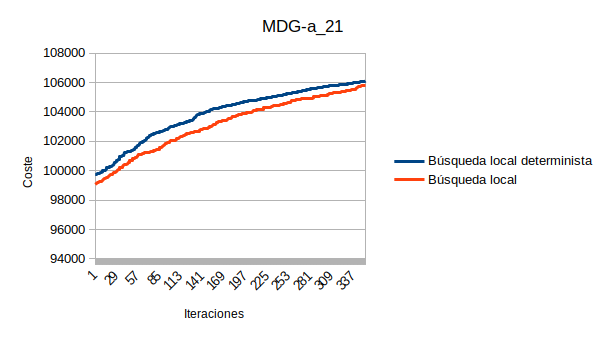
\includegraphics[scale=1]{../output/P1/MDG-a_21}
		%\caption{my-captino} \label{my-label}
	\end{figure}
	
	\begin{figure}[H] 
		\centering
		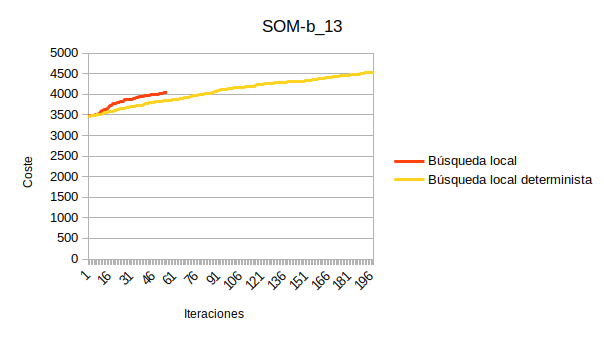
\includegraphics[scale=1]{../output/P1/SOM-b_13}%\caption{my-captino} \label{my-label}
	\end{figure}

	\paragraph{ Análisis } \ \\
	
	Podemos ver como en los distintos casos la evolución es particularmente distinta. Por un lado, para $MDG-a_21$ la convergencia de ambos algoritmos es asintóticamente idéntica, manteniéndose la $BLD$ por encima en parte debido a la solución inicial ligeramente mejor.Por otro, en $SOM-b_13$ la mejora de la $BL$ respecto a la $BLD$ es sustancial pero esta se estanca rápidamente debido a que su exploración del espacio es peor. Este es otro ejemplo de como los mismos algoritmos pueden comportarse de formas completamente distintas para entradas diferentes.

	\subsection{ Práctica 2 } \label{sec62}
	
	\subsubsection{ Experimento 1: resultados iniciales}
	
	Para este primer experimento se han estudiado los dos AGG, los dos AGE y los tres AM definidos anteriormente. Utilizando los parámetros definidos en \ref{procedimiento2}, lanzamos los algoritmos 30 veces por test-case cada uno y tomamos datos del tiempo, fitness y generaciones realizadas por cada uno. Presentamos a continuación las medias de estos datos:
	
	\begin{table}[H]
		\begin{tabular}{l|l|l|l|l|l|l|l|}
			\cline{2-8}
			& AGGu    & AGGp    & AGEu    & AGEp    & AM0     & AM1     & AM1     \\ \hline
			\multicolumn{1}{|l|}{MDG-a\_1}  & 108891  & 103366  & 109277  & 104244  & 110992  & 111932  & 111256  \\ \hline
			\multicolumn{1}{|l|}{MDG-a\_2}  & 108830  & 103784  & 109242  & 104577  & 111723  & 111468  & 111536  \\ \hline
			\multicolumn{1}{|l|}{MDG-a\_3}  & 108791  & 103647  & 109261  & 103492  & 111620  & 111296  & 111484  \\ \hline
			\multicolumn{1}{|l|}{MDG-a\_4}  & 108841  & 103714  & 109291  & 103558  & 111886  & 111738  & 111445  \\ \hline
			\multicolumn{1}{|l|}{MDG-a\_5}  & 108549  & 104275  & 109292  & 104132  & 111356  & 111566  & 111216  \\ \hline
			\multicolumn{1}{|l|}{MDG-a\_6}  & 108694  & 104393  & 109093  & 104210  & 111372  & 111768  & 111441  \\ \hline
			\multicolumn{1}{|l|}{MDG-a\_7}  & 108899  & 103750  & 109418  & 104317  & 111176  & 111125  & 111759  \\ \hline
			\multicolumn{1}{|l|}{MDG-a\_8}  & 108681  & 103860  & 109045  & 104168  & 111723  & 111738  & 111092  \\ \hline
			\multicolumn{1}{|l|}{MDG-a\_9}  & 108659  & 104258  & 109435  & 103738  & 111401  & 111734  & 111257  \\ \hline
			\multicolumn{1}{|l|}{MDG-a\_10} & 108775  & 102935  & 109155  & 104006  & 111837  & 110936  & 111396  \\ \hline
			\multicolumn{1}{|l|}{SOM-b\_11} & 20206.7 & 19432   & 20268   & 19401   & 20409.5 & 20371   & 20333.5 \\ \hline
			\multicolumn{1}{|l|}{SOM-b\_12} & 35246.8 & 34127.5 & 35340.9 & 34216   & 35432   & 35379.5 & 35372.5 \\ \hline
			\multicolumn{1}{|l|}{SOM-b\_13} & 4333.85 & 4049.5  & 4368.15 & 4148    & 4435    & 4484    & 4444    \\ \hline
			\multicolumn{1}{|l|}{SOM-b\_14} & 16305.5 & 15547.5 & 16424.2 & 15521.5 & 16623   & 16477   & 16582.5 \\ \hline
			\multicolumn{1}{|l|}{SOM-b\_15} & 35615.8 & 34058   & 35647.8 & 34386   & 35622.5 & 35846   & 35817.5 \\ \hline
			\multicolumn{1}{|l|}{SOM-b\_16} & 61871.5 & 59912.5 & 61995.1 & 60079.5 & 62317   & 62406.5 & 62044   \\ \hline
			\multicolumn{1}{|l|}{SOM-b\_17} & 6605.75 & 6290.5  & 6694.45 & 6289    & 6876.5  & 6904    & 6749.5  \\ \hline
			\multicolumn{1}{|l|}{SOM-b\_18} & 25023.5 & 23966   & 25206   & 23889.5 & 25259   & 25481   & 25396   \\ \hline
			\multicolumn{1}{|l|}{SOM-b\_19} & 54865.7 & 53187   & 55060.9 & 52865.5 & 55603   & 55468   & 55556   \\ \hline
			\multicolumn{1}{|l|}{SOM-b\_20} & 95792.9 & 92998.5 & 96038.6 & 93193   & 96319.5 & 96633.5 & 96542.5 \\ \hline
			\multicolumn{1}{|l|}{GKD-c\_21} & 17608.8 & 17017   & 17645.8 & 17128.3 & 17915.9 & 17899.7 & 17918.7 \\ \hline
			\multicolumn{1}{|l|}{GKD-c\_22} & 17756.5 & 17155.2 & 17834   & 17138.8 & 18112.5 & 17973.1 & 17888.4 \\ \hline
			\multicolumn{1}{|l|}{GKD-c\_23} & 17718   & 16929   & 17732.2 & 17027.1 & 17857.5 & 17968.2 & 17932.2 \\ \hline
			\multicolumn{1}{|l|}{GKD-c\_24} & 17749.5 & 16981.2 & 17746.4 & 17104.2 & 17791.6 & 17749.5 & 17963.5 \\ \hline
			\multicolumn{1}{|l|}{GKD-c\_25} & 17658.9 & 16816.9 & 17697.5 & 16992.3 & 17864.3 & 17820   & 17833.4 \\ \hline
			\multicolumn{1}{|l|}{GKD-c\_26} & 17582.4 & 17116.2 & 17615.8 & 17145.5 & 17856.2 & 17790.8 & 17843.8 \\ \hline
			\multicolumn{1}{|l|}{GKD-c\_27} & 17810   & 17096.8 & 17850.3 & 17070.8 & 17977.6 & 18038.6 & 17998.8 \\ \hline
			\multicolumn{1}{|l|}{GKD-c\_28} & 17649.3 & 17063   & 17734.5 & 17089.3 & 17948.9 & 18002.1 & 17819.3 \\ \hline
			\multicolumn{1}{|l|}{GKD-c\_29} & 17414.2 & 16761   & 17454.3 & 16822.8 & 17639.5 & 17532.5 & 17543.2 \\ \hline
			\multicolumn{1}{|l|}{GKD-c\_30} & 17721.8 & 16915.6 & 17706.5 & 17085.6 & 17850.2 & 17969.3 & 17963.6 \\ \hline
		\end{tabular}
		\caption{ Experimento 1 - Costes }
		\label{211}
	\end{table}

	\begin{table}[H]
		\begin{tabular}{l|l|l|l|l|l|l|l|}
			\cline{2-8}
			& AGGu     & AGGp     & AGEu     & AGEp     & AM0      & AM1      & AM1      \\ \hline
			\multicolumn{1}{|l|}{MDG-a\_1}  & 24.4233  & 23.8637  & 24.1219  & 23.6219  & 21.9402  & 23.2932  & 22.797   \\ \hline
			\multicolumn{1}{|l|}{MDG-a\_2}  & 24.405   & 23.8894  & 24.2071  & 23.4312  & 22.0997  & 22.2993  & 23.3811  \\ \hline
			\multicolumn{1}{|l|}{MDG-a\_3}  & 24.3328  & 23.852   & 24.3339  & 23.8606  & 23.2322  & 23.1624  & 23.1435  \\ \hline
			\multicolumn{1}{|l|}{MDG-a\_4}  & 24.3705  & 23.9463  & 24.1634  & 23.3537  & 22.8015  & 23.107   & 23.0078  \\ \hline
			\multicolumn{1}{|l|}{MDG-a\_5}  & 24.4211  & 23.7319  & 24.2868  & 23.9673  & 21.8929  & 22.533   & 22.8683  \\ \hline
			\multicolumn{1}{|l|}{MDG-a\_6}  & 24.4364  & 24.5861  & 24.3023  & 23.8618  & 22.3339  & 22.3768  & 23.0249  \\ \hline
			\multicolumn{1}{|l|}{MDG-a\_7}  & 24.3507  & 24.0536  & 24.1702  & 23.6154  & 22.6294  & 22.3369  & 23.1606  \\ \hline
			\multicolumn{1}{|l|}{MDG-a\_8}  & 24.4853  & 23.6647  & 24.0161  & 23.2876  & 22.6126  & 22.6438  & 22.8375  \\ \hline
			\multicolumn{1}{|l|}{MDG-a\_9}  & 24.4153  & 23.7216  & 24.2415  & 24.2212  & 22.7098  & 22.8243  & 21.8571  \\ \hline
			\multicolumn{1}{|l|}{MDG-a\_10} & 24.3466  & 23.4462  & 24.1385  & 24.1119  & 22.6193  & 22.8244  & 22.7726  \\ \hline
			\multicolumn{1}{|l|}{SOM-b\_11} & 1.20194  & 1.18055  & 1.20846  & 1.1629   & 1.24611  & 1.20307  & 1.20698  \\ \hline
			\multicolumn{1}{|l|}{SOM-b\_12} & 1.59528  & 1.53491  & 1.57967  & 1.58228  & 1.94155  & 1.61071  & 1.58557  \\ \hline
			\multicolumn{1}{|l|}{SOM-b\_13} & 0.868631 & 0.812625 & 0.857292 & 0.891678 & 0.438967 & 0.734924 & 0.853313 \\ \hline
			\multicolumn{1}{|l|}{SOM-b\_14} & 1.5129   & 1.48241  & 1.47245  & 1.42183  & 1.22705  & 1.41789  & 1.48675  \\ \hline
			\multicolumn{1}{|l|}{SOM-b\_15} & 2.09646  & 2.00823  & 2.08278  & 2.19775  & 2.40745  & 2.12159  & 2.08059  \\ \hline
			\multicolumn{1}{|l|}{SOM-b\_16} & 2.76473  & 2.65904  & 2.72259  & 2.68241  & 3.72652  & 2.86986  & 2.78566  \\ \hline
			\multicolumn{1}{|l|}{SOM-b\_17} & 1.37386  & 1.30215  & 1.3465   & 1.32537  & 0.740074 & 1.19312  & 1.35607  \\ \hline
			\multicolumn{1}{|l|}{SOM-b\_18} & 2.35214  & 2.22628  & 2.29393  & 2.21181  & 2.1313   & 2.30068  & 2.35398  \\ \hline
			\multicolumn{1}{|l|}{SOM-b\_19} & 3.30494  & 3.23536  & 3.29586  & 3.2272   & 4.0674   & 3.36809  & 3.38204  \\ \hline
			\multicolumn{1}{|l|}{SOM-b\_20} & 4.31045  & 4.23414  & 4.30605  & 4.14887  & 5.91416  & 4.61186  & 4.42713  \\ \hline
			\multicolumn{1}{|l|}{GKD-c\_21} & 1.36727  & 1.32412  & 1.35354  & 1.25208  & 0.765945 & 1.2595   & 1.33338  \\ \hline
			\multicolumn{1}{|l|}{GKD-c\_22} & 1.3738   & 1.30634  & 1.35173  & 1.24574  & 0.728988 & 1.20548  & 1.31984  \\ \hline
			\multicolumn{1}{|l|}{GKD-c\_23} & 1.37431  & 1.28311  & 1.35425  & 1.33676  & 0.767462 & 1.25363  & 1.33645  \\ \hline
			\multicolumn{1}{|l|}{GKD-c\_24} & 1.35535  & 1.3561   & 1.33929  & 1.31544  & 0.751525 & 1.16892  & 1.34858  \\ \hline
			\multicolumn{1}{|l|}{GKD-c\_25} & 1.36712  & 1.27663  & 1.33415  & 1.32144  & 0.733905 & 1.225    & 1.34138  \\ \hline
			\multicolumn{1}{|l|}{GKD-c\_26} & 1.37671  & 1.34339  & 1.35847  & 1.33036  & 0.740275 & 1.25453  & 1.38125  \\ \hline
			\multicolumn{1}{|l|}{GKD-c\_27} & 1.39016  & 1.31565  & 1.34685  & 1.30794  & 0.768023 & 1.18297  & 1.41582  \\ \hline
			\multicolumn{1}{|l|}{GKD-c\_28} & 1.37054  & 1.34797  & 1.33595  & 1.27007  & 0.732937 & 1.20843  & 1.31878  \\ \hline
			\multicolumn{1}{|l|}{GKD-c\_29} & 1.34627  & 1.30072  & 1.36707  & 1.29795  & 0.754039 & 1.23594  & 1.4178   \\ \hline
			\multicolumn{1}{|l|}{GKD-c\_30} & 1.33805  & 1.30159  & 1.34684  & 1.32056  & 0.751667 & 1.19237  & 1.31282  \\ \hline
		\end{tabular}
		\caption{ Experimento 1 - Tiempos (s) }
		\label{212}
	\end{table}

	\begin{table}[H]
		\begin{tabular}{l|l|l|l|l|l|l|l|}
			\cline{2-8}
			& AGGu    & AGGp   & AGEu  & AGEp  & AM0    & AM1    & AM1    \\ \hline
			\multicolumn{1}{|l|}{MDG-a\_1}  & 1997.5  & 1995.5 & 24975 & 24975 & 1320.5 & 1904.5 & 1980   \\ \hline
			\multicolumn{1}{|l|}{MDG-a\_2}  & 1996.35 & 1997   & 24975 & 24975 & 1368.5 & 1906   & 1976.5 \\ \hline
			\multicolumn{1}{|l|}{MDG-a\_3}  & 1997.75 & 1997   & 24975 & 24975 & 1357   & 1904   & 1976.5 \\ \hline
			\multicolumn{1}{|l|}{MDG-a\_4}  & 1995.6  & 1996   & 24975 & 24975 & 1370.5 & 1903   & 1974.5 \\ \hline
			\multicolumn{1}{|l|}{MDG-a\_5}  & 1997.3  & 1995.5 & 24975 & 24975 & 1328   & 1908.5 & 1976.5 \\ \hline
			\multicolumn{1}{|l|}{MDG-a\_6}  & 1996.3  & 1996   & 24975 & 24975 & 1340   & 1897   & 1969   \\ \hline
			\multicolumn{1}{|l|}{MDG-a\_7}  & 1997.9  & 1998   & 24975 & 24975 & 1328   & 1903   & 1978   \\ \hline
			\multicolumn{1}{|l|}{MDG-a\_8}  & 1997.6  & 1999.5 & 24975 & 24975 & 1334   & 1902   & 1979   \\ \hline
			\multicolumn{1}{|l|}{MDG-a\_9}  & 1997    & 1992.5 & 24975 & 24975 & 1369   & 1903.5 & 1977.5 \\ \hline
			\multicolumn{1}{|l|}{MDG-a\_10} & 1997.8  & 2001   & 24975 & 24975 & 1348   & 1902.5 & 1975.5 \\ \hline
			\multicolumn{1}{|l|}{SOM-b\_11} & 1997.55 & 1992.5 & 24975 & 24975 & 1020   & 1826.5 & 1955.5 \\ \hline
			\multicolumn{1}{|l|}{SOM-b\_12} & 1996.75 & 1994   & 24975 & 24975 & 1139.5 & 1866.5 & 1963.5 \\ \hline
			\multicolumn{1}{|l|}{SOM-b\_13} & 1995.8  & 1995.5 & 24975 & 24975 & 591    & 1624   & 1910   \\ \hline
			\multicolumn{1}{|l|}{SOM-b\_14} & 1997.45 & 1994   & 24975 & 24975 & 873.5  & 1794.5 & 1949   \\ \hline
			\multicolumn{1}{|l|}{SOM-b\_15} & 1995.45 & 1997   & 24975 & 24975 & 1115   & 1856   & 1965.5 \\ \hline
			\multicolumn{1}{|l|}{SOM-b\_16} & 1997.45 & 1998   & 24975 & 24975 & 1340   & 1896.5 & 1980   \\ \hline
			\multicolumn{1}{|l|}{SOM-b\_17} & 1996.2  & 1993.5 & 24975 & 24975 & 668    & 1696.5 & 1927   \\ \hline
			\multicolumn{1}{|l|}{SOM-b\_18} & 1995.5  & 1995   & 24975 & 24975 & 1025   & 1824.5 & 1958.5 \\ \hline
			\multicolumn{1}{|l|}{SOM-b\_19} & 1997.1  & 1994   & 24975 & 24975 & 1310   & 1894   & 1974.5 \\ \hline
			\multicolumn{1}{|l|}{SOM-b\_20} & 1997.55 & 1997   & 24975 & 24975 & 1372   & 1908.5 & 1971.5 \\ \hline
			\multicolumn{1}{|l|}{GKD-c\_21} & 1997.3  & 1995.5 & 24975 & 24975 & 704.5  & 1699.5 & 1929.5 \\ \hline
			\multicolumn{1}{|l|}{GKD-c\_22} & 1996.6  & 2000   & 24975 & 24975 & 675    & 1694   & 1922   \\ \hline
			\multicolumn{1}{|l|}{GKD-c\_23} & 1995    & 1995   & 24975 & 24975 & 705    & 1689   & 1928.5 \\ \hline
			\multicolumn{1}{|l|}{GKD-c\_24} & 1997.1  & 1996.5 & 24975 & 24975 & 720    & 1706   & 1928   \\ \hline
			\multicolumn{1}{|l|}{GKD-c\_25} & 1995.6  & 1997.5 & 24975 & 24975 & 680    & 1692.5 & 1925   \\ \hline
			\multicolumn{1}{|l|}{GKD-c\_26} & 1997.1  & 1992.5 & 24975 & 24975 & 679.5  & 1693   & 1918.5 \\ \hline
			\multicolumn{1}{|l|}{GKD-c\_27} & 1994.9  & 1997   & 24975 & 24975 & 699    & 1688   & 1925.5 \\ \hline
			\multicolumn{1}{|l|}{GKD-c\_28} & 1998.4  & 1997.5 & 24975 & 24975 & 670    & 1685.5 & 1917   \\ \hline
			\multicolumn{1}{|l|}{GKD-c\_29} & 1996.05 & 1995.5 & 24975 & 24975 & 681.5  & 1695.5 & 1922   \\ \hline
			\multicolumn{1}{|l|}{GKD-c\_30} & 1996.65 & 1994   & 24975 & 24975 & 700.5  & 1698.5 & 1924   \\ \hline
		\end{tabular}
		\caption{ Experimento 1 - Generaciones }
		\label{213}
	\end{table}

	\begin{table}[H]
		\begin{tabular}{l|l|l|l|l|l|l|l|}
			\cline{2-8}
			& AGGu    & AGGp    & AGEu     & AGEp     & AM0     & AM1     & AM2     \\ \hline
			\multicolumn{1}{|l|}{Desv}         & 5,93    & 9,84    & 5,56     & 9,56     & 4,33    & 4,27    & 4,44    \\ \hline
			\multicolumn{1}{|l|}{Tiempo (s)}   & 9,30    & 9,09    & 9,22     & 9,04     & 8,54    & 8,70    & 8,80    \\ \hline
			\multicolumn{1}{|l|}{Generaciones} & 1996,75 & 1995,98 & 24975,00 & 24975,00 & 1027,75 & 1805,43 & 1951,93 \\ \hline
		\end{tabular}
		\caption{ Experimento 1 - Comparativa entre algoritmos }
		\label{214}
	\end{table}

	\paragraph{ Análisis} \ \\
	
	Comencemos observando la tabla \ref{214} para obtener una \textbf{visión general} de los resultados obtenidos. Podemos apreciar consultando la fila $Desv$ que los algoritmos que mejores resultados obtienen son siempre los meméticos. En cuanto a los genéticos, tanto en la estrategia generacional como en la estacionaria el resultado es claro: el operador de cruce uniforme es notablemente mejor que el posicional (al menos combinándolo con el resto de operadores implementados y para los parámetros utilizados). Es por ello que en futuros experimentos no  estudiaremos ni AGGp ni AGEp. \\
	
	En cuanto a los \textbf{tiempos}, los resultados son realmente consistentes. Si bien los meméticos son un poco más rápidos, la diferencia no llegar a ser notable. Consultando la tabla \ref{212} vemos que para las entradas más grandes ($MDG$), los valores de todos los algoritmos oscilan entre 21 y 24 segundos. Ante tan breve variación podemos asumir que el "mejor" algoritmo será el que mejor valores obtenga, considerando que hemos fijado el número máximo de iteraciones. \\
	
	Volvemos a \ref{214} para observar el número medio de \textbf{generaciones} obtenido. En primer lugar puede parecer curioso que ambos algoritmos AGE obtengan exactamente el mismo valor medio. Adicionalmente, si observamos la tabla \ref{213} podemos ver como se obtienen 24975 generaciones para todos los experimentos (recordemos que este valor a su vez es una media entre 30 ejecuciones). Sin embargo, no podía ser de otra forma: el número de evaluaciones por generación de este algoritmos esta fijado de antemano, es exactamente dos. Considerando las 50 evaluaciones iniciales para inicializar la población, es lo esperado obtener exactamente $(50.000 - 50) / 2 = 24.975$ generaciones. \\
	
	Por otro lado, realizando una operación sencilla ( $n_evaluaciones / n_generaciones$) vemos que el número de evaluaciones por generación obtenido para los AGG oscila entorno a $2,5$. Los algoritmos meméticos obtienen valores parecidos exceptuando el $AM0$, que ejecuta la búsqueda local para toda la población cada 10 iteraciones, obtiene 5 una media aproximada de 5 evaluaciones por generación. \\
	
	Finalmente comparamos la eficacia de los algoritmos AGGu y AGEu. Para ello observamos la fila Desv en \ref{214} y los test-cases $MDG$ en la tabla \ref{211}. En ellos podemos ver como el AGEu obtiene valores ligeramente mayores que el AGGu en la mayoria de los casos. Sin embargo estos casos se encuentran realmente alejados de los mejores valores que oscilan entre $113.000$ y $114.000$, como podemos ver en la columna de óptimos de la tabla \ref{costes}. Como cabría esperar, todos los algoritmos meméticos obtienen mayores valores de $fitness$, siendo el mejor de ellos $AM1$, que aplicaba la búsqueda local a elementos arbitrarios de la población. \\
	
	De cara al siguiente experimento restringimos el conjunto de algoritmos estudiado al $AGEu$ y $AM1$, añadiendo la búsqueda local de la práctica anterior y el algoritmo memético mejorado.
	
	\subsubsection{ Experimento 2: Comparativa con práctica 1 y memético mejorado}
	
	En el experimento anterior utilizábamos unicamente los algoritmos obligatorios realizados en esta práctica para la comparación, de cara a evitar trabajar simultáneamente con nueve algoritmos distintos. Procedemos ahora a comparar los dos algoritmos que mejores resultados obtuvieron en el experimento anterior ($AGEu$ y $AM1$) con la búsqueda local que mejores resultados dio en la práctica anterior ($LSD$), junto con el algoritmo memético mejorado implementado para esta práctica. \\
	
	Para los algoritmos $AGEu$ y $AM1$ utilizamos los datos obtenidos en el experimento anterior, mientras que para la $LSD$ no tomaremos muestras de las evaluaciones realizadas ya que no tiene sentido compararlas con las generaciones de un algoritmo genético. \\
	
	\begin{table}[H]
		\centering
		\begin{tabular}{l|l|l|l|l|}
			\cline{2-5}
			& AGEu    & AM1     & AMM     & LSD     \\ \hline
			\multicolumn{1}{|l|}{MDG-a\_1}  & 109277  & 111932  & 111603  & 105344  \\ \hline
			\multicolumn{1}{|l|}{MDG-a\_2}  & 109242  & 111468  & 111771  & 106374  \\ \hline
			\multicolumn{1}{|l|}{MDG-a\_3}  & 109261  & 111296  & 111254  & 106137  \\ \hline
			\multicolumn{1}{|l|}{MDG-a\_4}  & 109291  & 111738  & 111930  & 106058  \\ \hline
			\multicolumn{1}{|l|}{MDG-a\_5}  & 109292  & 111566  & 111902  & 106222  \\ \hline
			\multicolumn{1}{|l|}{MDG-a\_6}  & 109093  & 111768  & 111227  & 106156  \\ \hline
			\multicolumn{1}{|l|}{MDG-a\_7}  & 109418  & 111125  & 111918  & 106126  \\ \hline
			\multicolumn{1}{|l|}{MDG-a\_8}  & 109045  & 111738  & 111388  & 105580  \\ \hline
			\multicolumn{1}{|l|}{MDG-a\_9}  & 109435  & 111734  & 111247  & 106000  \\ \hline
			\multicolumn{1}{|l|}{MDG-a\_10} & 109155  & 110936  & 111274  & 105870  \\ \hline
			\multicolumn{1}{|l|}{SOM-b\_11} & 20268   & 20371   & 20595   & 20615.5 \\ \hline
			\multicolumn{1}{|l|}{SOM-b\_12} & 35340.9 & 35379.5 & 35698.5 & 35745   \\ \hline
			\multicolumn{1}{|l|}{SOM-b\_13} & 4368.15 & 4484    & 4556    & 4610    \\ \hline
			\multicolumn{1}{|l|}{SOM-b\_14} & 16424.2 & 16477   & 16882.5 & 16881   \\ \hline
			\multicolumn{1}{|l|}{SOM-b\_15} & 35647.8 & 35846   & 36100.5 & 36130   \\ \hline
			\multicolumn{1}{|l|}{SOM-b\_16} & 61995.1 & 62406.5 & 62670.5 & 62332.5 \\ \hline
			\multicolumn{1}{|l|}{SOM-b\_17} & 6694.45 & 6904    & 6914    & 6992    \\ \hline
			\multicolumn{1}{|l|}{SOM-b\_18} & 25206   & 25481   & 25764   & 25396   \\ \hline
			\multicolumn{1}{|l|}{SOM-b\_19} & 55060.9 & 55468   & 55845   & 55189   \\ \hline
			\multicolumn{1}{|l|}{SOM-b\_20} & 96038.6 & 96633.5 & 96832.5 & 95558   \\ \hline
			\multicolumn{1}{|l|}{GKD-c\_21} & 17645.8 & 17899.7 & 18048.3 & 18046   \\ \hline
			\multicolumn{1}{|l|}{GKD-c\_22} & 17834   & 17973.1 & 18206.8 & 18208.6 \\ \hline
			\multicolumn{1}{|l|}{GKD-c\_23} & 17732.2 & 17968.2 & 18001.7 & 18032.2 \\ \hline
			\multicolumn{1}{|l|}{GKD-c\_24} & 17746.4 & 17749.5 & 18051   & 18035.9 \\ \hline
			\multicolumn{1}{|l|}{GKD-c\_25} & 17697.5 & 17820   & 18001.9 & 18041   \\ \hline
			\multicolumn{1}{|l|}{GKD-c\_26} & 17615.8 & 17790.8 & 17945.6 & 17977.3 \\ \hline
			\multicolumn{1}{|l|}{GKD-c\_27} & 17850.3 & 18038.6 & 18121.5 & 18164.7 \\ \hline
			\multicolumn{1}{|l|}{GKD-c\_28} & 17734.5 & 18002.1 & 18085.8 & 18109.2 \\ \hline
			\multicolumn{1}{|l|}{GKD-c\_29} & 17454.3 & 17532.5 & 17809.5 & 17825.9 \\ \hline
			\multicolumn{1}{|l|}{GKD-c\_30} & 17706.5 & 17969.3 & 18045.5 & 18030.4 \\ \hline
		\end{tabular}
		\caption{ Experimento 2 - Costes }
		\label{221}
	\end{table}
	
	\begin{table}[H]
		\centering
		\begin{tabular}{l|l|l|l|l|}
			\cline{2-5}
			& AGEu     & AM1      & AMM      & LSD       \\ \hline
			\multicolumn{1}{|l|}{MDG-a\_1}  & 24.1219  & 23.2932  & 12.9742  & 1.36342   \\ \hline
			\multicolumn{1}{|l|}{MDG-a\_2}  & 24.2071  & 22.2993  & 13.3091  & 1.6805    \\ \hline
			\multicolumn{1}{|l|}{MDG-a\_3}  & 24.3339  & 23.1624  & 13.1407  & 1.6231    \\ \hline
			\multicolumn{1}{|l|}{MDG-a\_4}  & 24.1634  & 23.107   & 13.5073  & 1.47381   \\ \hline
			\multicolumn{1}{|l|}{MDG-a\_5}  & 24.2868  & 22.533   & 13.3399  & 1.3582    \\ \hline
			\multicolumn{1}{|l|}{MDG-a\_6}  & 24.3023  & 22.3768  & 13.4465  & 1.34014   \\ \hline
			\multicolumn{1}{|l|}{MDG-a\_7}  & 24.1702  & 22.3369  & 13.1167  & 1.37532   \\ \hline
			\multicolumn{1}{|l|}{MDG-a\_8}  & 24.0161  & 22.6438  & 13.3501  & 1.37907   \\ \hline
			\multicolumn{1}{|l|}{MDG-a\_9}  & 24.2415  & 22.8243  & 13.5913  & 1.4398    \\ \hline
			\multicolumn{1}{|l|}{MDG-a\_10} & 24.1385  & 22.8244  & 13.3084  & 1.15298   \\ \hline
			\multicolumn{1}{|l|}{SOM-b\_11} & 1.20846  & 1.20307  & 0.744437 & 0.108794  \\ \hline
			\multicolumn{1}{|l|}{SOM-b\_12} & 1.57967  & 1.61071  & 1.15973  & 0.207137  \\ \hline
			\multicolumn{1}{|l|}{SOM-b\_13} & 0.857292 & 0.734924 & 0.379541 & 0.0220685 \\ \hline
			\multicolumn{1}{|l|}{SOM-b\_14} & 1.47245  & 1.41789  & 0.791695 & 0.120156  \\ \hline
			\multicolumn{1}{|l|}{SOM-b\_15} & 2.08278  & 2.12159  & 1.31182  & 0.31353   \\ \hline
			\multicolumn{1}{|l|}{SOM-b\_16} & 2.72259  & 2.86986  & 1.9723   & 0.515377  \\ \hline
			\multicolumn{1}{|l|}{SOM-b\_17} & 1.3465   & 1.19312  & 0.585186 & 0.0500965 \\ \hline
			\multicolumn{1}{|l|}{SOM-b\_18} & 2.29393  & 2.30068  & 1.23769  & 0.201794  \\ \hline
			\multicolumn{1}{|l|}{SOM-b\_19} & 3.29586  & 3.36809  & 2.07114  & 0.40222   \\ \hline
			\multicolumn{1}{|l|}{SOM-b\_20} & 4.30605  & 4.61186  & 3.05897  & 0.619741  \\ \hline
			\multicolumn{1}{|l|}{GKD-c\_21} & 1.35354  & 1.2595   & 0.594739 & 0.0729705 \\ \hline
			\multicolumn{1}{|l|}{GKD-c\_22} & 1.35173  & 1.20548  & 0.594813 & 0.0750675 \\ \hline
			\multicolumn{1}{|l|}{GKD-c\_23} & 1.35425  & 1.25363  & 0.574288 & 0.0886425 \\ \hline
			\multicolumn{1}{|l|}{GKD-c\_24} & 1.33929  & 1.16892  & 0.593927 & 0.079868  \\ \hline
			\multicolumn{1}{|l|}{GKD-c\_25} & 1.33415  & 1.225    & 0.590534 & 0.0821845 \\ \hline
			\multicolumn{1}{|l|}{GKD-c\_26} & 1.35847  & 1.25453  & 0.602524 & 0.0644635 \\ \hline
			\multicolumn{1}{|l|}{GKD-c\_27} & 1.34685  & 1.18297  & 0.582689 & 0.0856165 \\ \hline
			\multicolumn{1}{|l|}{GKD-c\_28} & 1.33595  & 1.20843  & 0.600887 & 0.0891885 \\ \hline
			\multicolumn{1}{|l|}{GKD-c\_29} & 1.36707  & 1.23594  & 0.590709 & 0.06394   \\ \hline
			\multicolumn{1}{|l|}{GKD-c\_30} & 1.34684  & 1.19237  & 0.593216 & 0.091104  \\ \hline
		\end{tabular}
		\caption{ Experimento 2 - Tiempos (s) }
		\label{222}
	\end{table}	
	
	\begin{table}[H]
		\centering
		\begin{tabular}{l|l|l|l|}
			\cline{2-4}
			& AGEu  & AM1    & AMM   \\ \hline
			\multicolumn{1}{|l|}{MDG-a\_1}  & 24975 & 1904.5 & 770   \\ \hline
			\multicolumn{1}{|l|}{MDG-a\_2}  & 24975 & 1906   & 770   \\ \hline
			\multicolumn{1}{|l|}{MDG-a\_3}  & 24975 & 1904   & 770.5 \\ \hline
			\multicolumn{1}{|l|}{MDG-a\_4}  & 24975 & 1903   & 770   \\ \hline
			\multicolumn{1}{|l|}{MDG-a\_5}  & 24975 & 1908.5 & 770   \\ \hline
			\multicolumn{1}{|l|}{MDG-a\_6}  & 24975 & 1897   & 770   \\ \hline
			\multicolumn{1}{|l|}{MDG-a\_7}  & 24975 & 1903   & 770   \\ \hline
			\multicolumn{1}{|l|}{MDG-a\_8}  & 24975 & 1902   & 770   \\ \hline
			\multicolumn{1}{|l|}{MDG-a\_9}  & 24975 & 1903.5 & 770   \\ \hline
			\multicolumn{1}{|l|}{MDG-a\_10} & 24975 & 1902.5 & 770   \\ \hline
			\multicolumn{1}{|l|}{SOM-b\_11} & 24975 & 1826.5 & 810   \\ \hline
			\multicolumn{1}{|l|}{SOM-b\_12} & 24975 & 1866.5 & 945   \\ \hline
			\multicolumn{1}{|l|}{SOM-b\_13} & 24975 & 1624   & 795   \\ \hline
			\multicolumn{1}{|l|}{SOM-b\_14} & 24975 & 1794.5 & 824.5 \\ \hline
			\multicolumn{1}{|l|}{SOM-b\_15} & 24975 & 1856   & 810   \\ \hline
			\multicolumn{1}{|l|}{SOM-b\_16} & 24975 & 1896.5 & 780   \\ \hline
			\multicolumn{1}{|l|}{SOM-b\_17} & 24975 & 1696.5 & 776   \\ \hline
			\multicolumn{1}{|l|}{SOM-b\_18} & 24975 & 1824.5 & 770   \\ \hline
			\multicolumn{1}{|l|}{SOM-b\_19} & 24975 & 1894   & 775.5 \\ \hline
			\multicolumn{1}{|l|}{SOM-b\_20} & 24975 & 1908.5 & 770   \\ \hline
			\multicolumn{1}{|l|}{GKD-c\_21} & 24975 & 1699.5 & 775.5 \\ \hline
			\multicolumn{1}{|l|}{GKD-c\_22} & 24975 & 1694   & 772   \\ \hline
			\multicolumn{1}{|l|}{GKD-c\_23} & 24975 & 1689   & 777   \\ \hline
			\multicolumn{1}{|l|}{GKD-c\_24} & 24975 & 1706   & 776.5 \\ \hline
			\multicolumn{1}{|l|}{GKD-c\_25} & 24975 & 1692.5 & 771   \\ \hline
			\multicolumn{1}{|l|}{GKD-c\_26} & 24975 & 1693   & 771   \\ \hline
			\multicolumn{1}{|l|}{GKD-c\_27} & 24975 & 1688   & 778   \\ \hline
			\multicolumn{1}{|l|}{GKD-c\_28} & 24975 & 1685.5 & 776   \\ \hline
			\multicolumn{1}{|l|}{GKD-c\_29} & 24975 & 1695.5 & 772.5 \\ \hline
			\multicolumn{1}{|l|}{GKD-c\_30} & 24975 & 1698.5 & 775   \\ \hline
		\end{tabular}
		\caption{ Experimento 2 - Generaciones }
		\label{223}
	\end{table}
	
	\begin{table}[H]
		\centering
		\begin{tabular}{l|l|l|l|l|}
			\cline{2-5}
			& AGEu     & AM1     & AMM    & LSD                    \\ \hline
			\multicolumn{1}{|l|}{Desv}         & 5,56     & 4,27    & 3,69   & 5,35                   \\ \hline
			\multicolumn{1}{|l|}{Tiempo (s)}   & 9,22     & 8,70    & 5,08   & 0,58                   \\ \hline
			\multicolumn{1}{|l|}{Generaciones} & 24975,00 & 1805,43 & 783,37 & \multicolumn{1}{c|}{-} \\ \hline
		\end{tabular}
		\caption{ Experimento 2 - Comparativa entre algoritmos }
		\label{224}
	\end{table}
	
	\paragraph{ Análisis } \ \\
	
	Comparando en primer lugar la $LSD$ con el resto de algoritmos, vemos en la tabla \ref{224} como obtenemos resultados ligeramente mejores que el $AGEu$, pero peores que el $AM1$. Sin embargo fijándonos en \ref{221} caso a caso vemos como para las entradas de tipo $MDG$ la búsqueda local obtiene valores considerablemente peores, mientras que en casos más reducidos queda por encima que el $AGEu$, como son las mayoría de los $SOM$ y $GKD$. Adicionalmente, los tiempos obtenidos para $LSD$ son ridículamente menores que los del resto de algoritmos. \\ 
	
	En resumen podríamos deducir que para problemas de tamaño reducido la búsqueda local obtiene no solo mejores resultados sino tiempos muchos menores que los algoritmos genéticos, mientras que para casos mayores tienen un rendimiento bastante reducido. \\
	
	Por otro lado, con el algoritmo memético mejorado observamos en \ref{224} que se obtiene un mejor valor de $Desv$, si bien mirando caso a caso en la tabla \ref{221} las soluciones no son notablemente mejores. Sin embargo si que se ha producido una mejora notable en cuanto a tiempos que se reducen casi un 50\% en los mayores casos. \\
	
	De igual forma que ocurría en el experimento 3 de la práctica anterior (\ref{exp13}), el cambio en la búsqueda propicia una convergencia notablemente más rápida, si bien los valores alcanzados no presentan grandes diferencias. De igual forma que hizo el experimento 3 en la práctica anterior, estos resultados propician otro experimento para estudiar la evolución de las soluciones a nivel generacional.

	\subsubsection{ Experimento 3: Estudio evolutivo a nivel generacional }

	Para este último experimento nos ceñimos a los algoritmos $AGEu$, $AM1$ y $AMM$. Así mismo utilizaremos unicamente dos conjuntos de datos, $MDG-a_21$ y $SOM-b_13$, por sus distintos tamaños. Realizamos una única ejecución para cada algoritmo por conjunto de datos. Presentamos dos gráficas distintas para cada conjunto de datos debido a la abismal diferencia en el número de generaciones.

	\begin{figure}[H] 
		\centering
		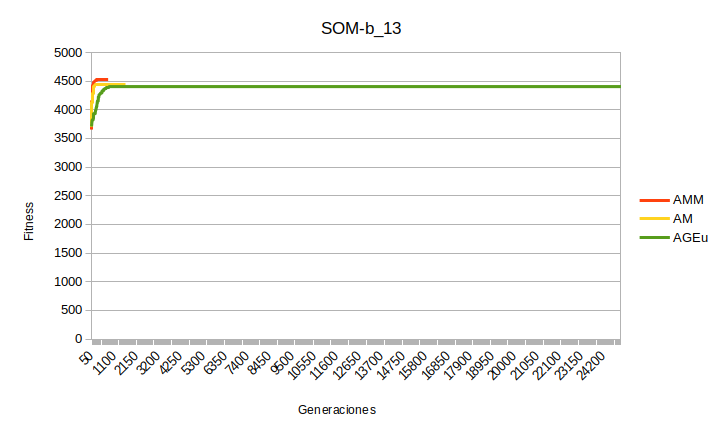
\includegraphics[scale=0.9]{../output/P2/exp3/SOM1}
		%\caption{my-captino} \label{my-label}
	\end{figure}
	
	\begin{figure}[H] 
		\centering
		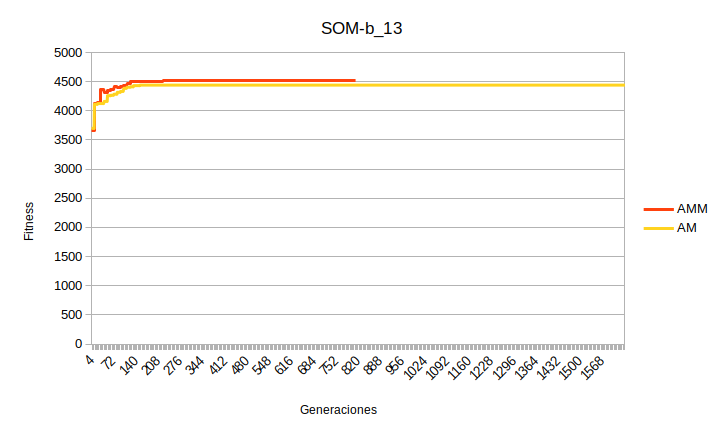
\includegraphics[scale=0.9]{../output/P2/exp3/SOM2}
		%\caption{my-captino} \label{my-label}
	\end{figure}
	
	\begin{figure}[H] 
		\centering
		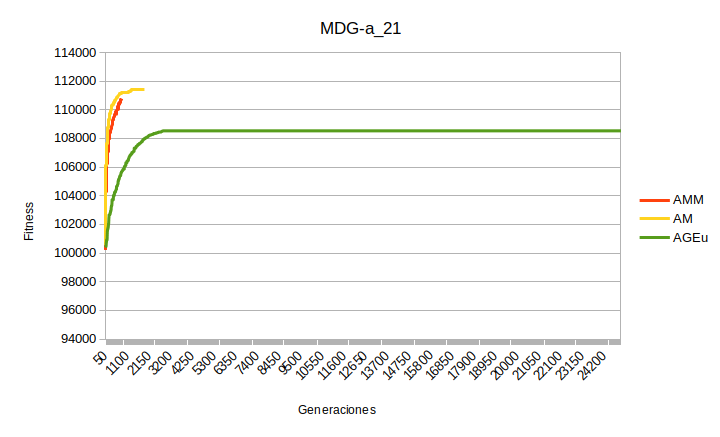
\includegraphics[scale=1]{../output/P2/exp3/MDG1}
		%\caption{my-captino} \label{my-label}
	\end{figure}
	
	\begin{figure}[H] 
		\centering
		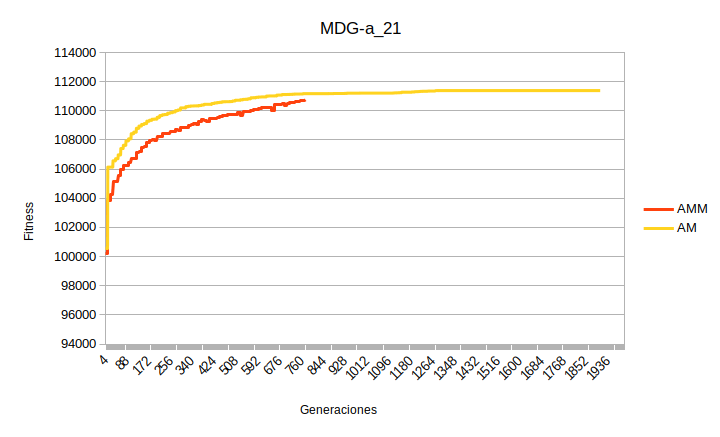
\includegraphics[scale=1]{../output/P2/exp3/MDG2}
		%\caption{my-captino} \label{my-label}
	\end{figure}

	
	\paragraph{ Análisis } \ \\
	
	Podemos observar claramente en ambos conjuntos de datos como la hipótesis formulada en el experimento anterior era parcialmente errónea: el algoritmo $AMM$ no converge más deprisa generacionalmente que el $AM$ sino que ambos lo hacen extremadamente rápido, de igual forma que el $AGEu$. Observar este hecho nos permitiría dirigir nuestros esfuerzos a diseñar y utilizar otros operadores para explorar más el espacio de soluciones y no estancarnos tan rápidamente. \\
	
	Aún así queda relativamente claro que quizás una estrategia evolutiva para este tipo de casos de prueba no sea el mejor procedimiento, ya que en general obtenemos tiempos mucho mayores que los de las búsquedas implementadas en la práctica anterior y si permitimos que las búsquedas exploren lo suficiente obtendremos resultados mejores y seguramente en un tiempo menor. Del mismo modo, para otros conjuntos de datos mayores que los utilizados las estrategias evolutivas podrían dar mejores resultados.

	\subsection{ Práctica 3 } \label{sec63}
	
	\subsubsection{ Experimento 1: resultados iniciales}

	Para este primer experimento se han ejecutado los 5 algoritmos sobre cada conjunto de datos un total de 5 veces, obteniendo la media para cada valor. Los parámetros utilizados han sido los definidos en la sección \ref{procedimiento3}. Presentamos a continuación los resultados obtenidos:
	
	\begin{table}[H]
		\centering
		\begin{tabular}{l|l|l|l|l|l|}
			\cline{2-6}
			& BMB & GRASP & ILS & ES & ILS-ES \\ \hline
			\multicolumn{1}{|l|}{MDG-a\_1} & 106602 & 106628 & 106739 & 110783 & 111503 \\ \hline
			\multicolumn{1}{|l|}{MDG-a\_2} & 106682 & 106720 & 106829 & 110755 & 111388 \\ \hline
			\multicolumn{1}{|l|}{MDG-a\_3} & 106660 & 106398 & 106479 & 110694 & 111477 \\ \hline
			\multicolumn{1}{|l|}{MDG-a\_4} & 106639 & 106556 & 106652 & 110849 & 111664 \\ \hline
			\multicolumn{1}{|l|}{MDG-a\_5} & 106941 & 106733 & 107043 & 110850 & 111436 \\ \hline
			\multicolumn{1}{|l|}{MDG-a\_6} & 106900 & 106950 & 106734 & 110886 & 111532 \\ \hline
			\multicolumn{1}{|l|}{MDG-a\_7} & 106719 & 106771 & 106715 & 110859 & 111674 \\ \hline
			\multicolumn{1}{|l|}{MDG-a\_8} & 106692 & 106577 & 106670 & 110765 & 111457 \\ \hline
			\multicolumn{1}{|l|}{MDG-a\_9} & 107308 & 107129 & 107195 & 110794 & 111483 \\ \hline
			\multicolumn{1}{|l|}{MDG-a\_10} & 106989 & 106792 & 106854 & 110809 & 111600 \\ \hline
			\multicolumn{1}{|l|}{SOM-b\_11} & 19379.4 & 19354.8 & 19485.8 & 20481.1 & 20511 \\ \hline
			\multicolumn{1}{|l|}{SOM-b\_12} & 34117.2 & 34050.2 & 34187.6 & 35462.4 & 35600 \\ \hline
			\multicolumn{1}{|l|}{SOM-b\_13} & 4142.4 & 4103.4 & 4124.4 & 4333.27 & 4385 \\ \hline
			\multicolumn{1}{|l|}{SOM-b\_14} & 15778 & 15727.2 & 15789.6 & 16441.1 & 16775.2 \\ \hline
			\multicolumn{1}{|l|}{SOM-b\_15} & 34282.4 & 34262.2 & 34324.2 & 36045.3 & 36098.6 \\ \hline
			\multicolumn{1}{|l|}{SOM-b\_16} & 60009 & 59923.6 & 60213 & 62444 & 62598.2 \\ \hline
			\multicolumn{1}{|l|}{SOM-b\_17} & 6415 & 6352.4 & 6386.6 & 6594.37 & 6740 \\ \hline
			\multicolumn{1}{|l|}{SOM-b\_18} & 24269.4 & 24268 & 24313.4 & 25258.2 & 25612.6 \\ \hline
			\multicolumn{1}{|l|}{SOM-b\_19} & 53094.8 & 53239.4 & 53296.8 & 55540.3 & 55755.8 \\ \hline
			\multicolumn{1}{|l|}{SOM-b\_20} & 93308.2 & 93132.8 & 93426.4 & 96713.9 & 96956.4 \\ \hline
			\multicolumn{1}{|l|}{GKD-c\_21} & 16998.2 & 16801.9 & 16916.1 & 17656.1 & 17766.7 \\ \hline
			\multicolumn{1}{|l|}{GKD-c\_22} & 17043.4 & 17043.2 & 17132.5 & 17828.3 & 17944.5 \\ \hline
			\multicolumn{1}{|l|}{GKD-c\_23} & 16901.6 & 16870.7 & 16854.2 & 17647.9 & 17839.5 \\ \hline
			\multicolumn{1}{|l|}{GKD-c\_24} & 16848.2 & 16713.3 & 16784.5 & 17549.3 & 17856.3 \\ \hline
			\multicolumn{1}{|l|}{GKD-c\_25} & 16952.7 & 16983.3 & 16985.4 & 17675.8 & 17794.3 \\ \hline
			\multicolumn{1}{|l|}{GKD-c\_26} & 16875 & 16850.2 & 16805.1 & 17574.5 & 17733.4 \\ \hline
			\multicolumn{1}{|l|}{GKD-c\_27} & 16966 & 16945.4 & 17025 & 17692.6 & 17931 \\ \hline
			\multicolumn{1}{|l|}{GKD-c\_28} & 16904.4 & 16792.9 & 16882.1 & 17584.4 & 17817.8 \\ \hline
			\multicolumn{1}{|l|}{GKD-c\_29} & 16792.4 & 16731.8 & 16819.9 & 17465.7 & 17533.8 \\ \hline
			\multicolumn{1}{|l|}{GKD-c\_30} & 16906 & 16882 & 17020.1 & 17638.2 & 17842 \\ \hline
		\end{tabular}	
		\caption{ Experimento 1 - Costes }
		\label{311}
	\end{table}
	
	\begin{table}[H]
		\centering
		\begin{tabular}{l|l|l|l|l|l|}
			\cline{2-6}
			& BMB & GRASP & ILS & ES & ILS-ES \\ \hline
			\multicolumn{1}{|l|}{MDG-a\_1} & 49.0739 & 59.0902 & 43.6282 & 0.0698885 & 1.79686 \\ \hline
			\multicolumn{1}{|l|}{MDG-a\_2} & 47.2971 & 58.2082 & 38.9329 & 0.0675791 & 1.84509 \\ \hline
			\multicolumn{1}{|l|}{MDG-a\_3} & 48.8751 & 60.4751 & 41.8564 & 0.0687969 & 1.84174 \\ \hline
			\multicolumn{1}{|l|}{MDG-a\_4} & 46.9536 & 59.2102 & 42.113 & 0.0671837 & 1.80902 \\ \hline
			\multicolumn{1}{|l|}{MDG-a\_5} & 46.4693 & 58.5162 & 40.1259 & 0.0711271 & 1.80773 \\ \hline
			\multicolumn{1}{|l|}{MDG-a\_6} & 50.6289 & 58.3947 & 39.3803 & 0.0696495 & 1.91803 \\ \hline
			\multicolumn{1}{|l|}{MDG-a\_7} & 50.0693 & 59.8216 & 42.261 & 0.0720882 & 1.96471 \\ \hline
			\multicolumn{1}{|l|}{MDG-a\_8} & 50.3327 & 57.4257 & 42.4366 & 0.0725582 & 1.85534 \\ \hline
			\multicolumn{1}{|l|}{MDG-a\_9} & 51.0673 & 57.9522 & 42.0621 & 0.0706882 & 1.81985 \\ \hline
			\multicolumn{1}{|l|}{MDG-a\_10} & 48.0246 & 55.7168 & 39.2987 & 0.0691525 & 1.80642 \\ \hline
			\multicolumn{1}{|l|}{SOM-b\_11} & 2.51987 & 2.58272 & 1.72957 & 0.0040066 & 0.0881496 \\ \hline
			\multicolumn{1}{|l|}{SOM-b\_12} & 5.08422 & 4.70358 & 3.60574 & 0.00564903 & 0.127036 \\ \hline
			\multicolumn{1}{|l|}{SOM-b\_13} & 0.779868 & 0.855719 & 0.717718 & 0.0017272 & 0.0436588 \\ \hline
			\multicolumn{1}{|l|}{SOM-b\_14} & 3.05045 & 2.93316 & 2.36924 & 0.0034138 & 0.0951466 \\ \hline
			\multicolumn{1}{|l|}{SOM-b\_15} & 5.561 & 7.07467 & 4.04161 & 0.00609723 & 0.154546 \\ \hline
			\multicolumn{1}{|l|}{SOM-b\_16} & 9.95388 & 9.18353 & 6.92641 & 0.00850483 & 0.214825 \\ \hline
			\multicolumn{1}{|l|}{SOM-b\_17} & 1.33494 & 1.52211 & 1.27639 & 0.002594 & 0.0670172 \\ \hline
			\multicolumn{1}{|l|}{SOM-b\_18} & 3.81373 & 4.48845 & 3.3468 & 0.0059226 & 0.154129 \\ \hline
			\multicolumn{1}{|l|}{SOM-b\_19} & 7.89786 & 8.4723 & 5.90613 & 0.0107726 & 0.249243 \\ \hline
			\multicolumn{1}{|l|}{SOM-b\_20} & 13.0212 & 13.8864 & 8.94794 & 0.0163185 & 0.367531 \\ \hline
			\multicolumn{1}{|l|}{GKD-c\_21} & 1.2892 & 1.37929 & 1.15655 & 0.0029151 & 0.0731608 \\ \hline
			\multicolumn{1}{|l|}{GKD-c\_22} & 1.70095 & 2.02773 & 1.49886 & 0.00312513 & 0.0822374 \\ \hline
			\multicolumn{1}{|l|}{GKD-c\_23} & 1.37259 & 1.58353 & 1.28942 & 0.00286893 & 0.075702 \\ \hline
			\multicolumn{1}{|l|}{GKD-c\_24} & 1.60498 & 1.71671 & 1.44737 & 0.0026749 & 0.0747024 \\ \hline
			\multicolumn{1}{|l|}{GKD-c\_25} & 1.45728 & 1.85319 & 1.10289 & 0.00291507 & 0.0696366 \\ \hline
			\multicolumn{1}{|l|}{GKD-c\_26} & 1.74943 & 1.75799 & 1.44904 & 0.0027906 & 0.0701662 \\ \hline
			\multicolumn{1}{|l|}{GKD-c\_27} & 1.87826 & 1.96778 & 1.60348 & 0.00258927 & 0.0718804 \\ \hline
			\multicolumn{1}{|l|}{GKD-c\_28} & 1.44559 & 1.82079 & 1.42973 & 0.0028796 & 0.0717026 \\ \hline
			\multicolumn{1}{|l|}{GKD-c\_29} & 1.68961 & 1.77564 & 1.6112 & 0.00327023 & 0.072215 \\ \hline
			\multicolumn{1}{|l|}{GKD-c\_30} & 1.64303 & 1.72296 & 1.49715 & 0.0029447 & 0.0697832 \\ \hline
		\end{tabular}
		\caption{ Experimento 1 - Tiempos }
		\label{312}
	\end{table}

	\begin{table}[H]
		\centering
		\begin{tabular}{l|l|l|l|l|l|}
			\cline{2-6}
			& BMB & GRASP & ILS & ES & ILS-ES \\ \hline
			\multicolumn{1}{|l|}{MDG-a\_1} & 328885 & 324626 & 314896 & 10119.3 & 260282 \\ \hline
			\multicolumn{1}{|l|}{MDG-a\_2} & 326150 & 320756 & 289330 & 10212.1 & 256595 \\ \hline
			\multicolumn{1}{|l|}{MDG-a\_3} & 334009 & 323001 & 304075 & 10468.4 & 258500 \\ \hline
			\multicolumn{1}{|l|}{MDG-a\_4} & 321895 & 328851 & 304389 & 10076.2 & 258344 \\ \hline
			\multicolumn{1}{|l|}{MDG-a\_5} & 319813 & 313591 & 300009 & 10472.4 & 258913 \\ \hline
			\multicolumn{1}{|l|}{MDG-a\_6} & 333750 & 328158 & 298332 & 10452.8 & 257328 \\ \hline
			\multicolumn{1}{|l|}{MDG-a\_7} & 334451 & 324339 & 310646 & 10480.4 & 260560 \\ \hline
			\multicolumn{1}{|l|}{MDG-a\_8} & 334695 & 321559 & 306633 & 10186.3 & 258781 \\ \hline
			\multicolumn{1}{|l|}{MDG-a\_9} & 349747 & 333679 & 302890 & 10293.2 & 257960 \\ \hline
			\multicolumn{1}{|l|}{MDG-a\_10} & 325557 & 314618 & 288949 & 10188.4 & 261783 \\ \hline
			\multicolumn{1}{|l|}{SOM-b\_11} & 177501 & 170742 & 123893 & 3583.47 & 78248.4 \\ \hline
			\multicolumn{1}{|l|}{SOM-b\_12} & 209891 & 188671 & 151402 & 4629.77 & 107787 \\ \hline
			\multicolumn{1}{|l|}{SOM-b\_13} & 205618 & 209657 & 194371 & 1216.67 & 28121 \\ \hline
			\multicolumn{1}{|l|}{SOM-b\_14} & 259971 & 242695 & 209893 & 2578 & 70670 \\ \hline
			\multicolumn{1}{|l|}{SOM-b\_15} & 229864 & 231782 & 170351 & 4695.23 & 116164 \\ \hline
			\multicolumn{1}{|l|}{SOM-b\_16} & 238926 & 208907 & 170419 & 6311.6 & 159232 \\ \hline
			\multicolumn{1}{|l|}{SOM-b\_17} & 233367 & 223202 & 224836 & 1465.23 & 38502 \\ \hline
			\multicolumn{1}{|l|}{SOM-b\_18} & 222063 & 223519 & 198029 & 3642.63 & 95055.2 \\ \hline
			\multicolumn{1}{|l|}{SOM-b\_19} & 211630 & 208604 & 166360 & 6704.03 & 152527 \\ \hline
			\multicolumn{1}{|l|}{SOM-b\_20} & 217283 & 208528 & 152350 & 9770.63 & 213407 \\ \hline
			\multicolumn{1}{|l|}{GKD-c\_21} & 220069 & 197173 & 204440 & 1609.33 & 39050.8 \\ \hline
			\multicolumn{1}{|l|}{GKD-c\_22} & 284421 & 322801 & 264848 & 1742.17 & 41579.4 \\ \hline
			\multicolumn{1}{|l|}{GKD-c\_23} & 238657 & 250522 & 214621 & 1621.23 & 41557.8 \\ \hline
			\multicolumn{1}{|l|}{GKD-c\_24} & 273074 & 257431 & 235181 & 1505.93 & 42126 \\ \hline
			\multicolumn{1}{|l|}{GKD-c\_25} & 253983 & 289182 & 189161 & 1623 & 40206.4 \\ \hline
			\multicolumn{1}{|l|}{GKD-c\_26} & 299757 & 275568 & 250453 & 1544.03 & 40141.6 \\ \hline
			\multicolumn{1}{|l|}{GKD-c\_27} & 317293 & 316005 & 277184 & 1439.33 & 41566.2 \\ \hline
			\multicolumn{1}{|l|}{GKD-c\_28} & 245675 & 284221 & 242515 & 1607.5 & 41367.4 \\ \hline
			\multicolumn{1}{|l|}{GKD-c\_29} & 284225 & 275966 & 271301 & 1862.17 & 41225.6 \\ \hline
			\multicolumn{1}{|l|}{GKD-c\_30} & 283055 & 277548 & 259134 & 1662.6 & 40248 \\ \hline
		\end{tabular}
		\caption{ Experimento 1 - Evaluaciones }
		\label{313}
	\end{table}

	\begin{table}[H]
		\centering
		\begin{tabular}{l|l|l|l|l|l|}
			\cline{2-6}
			& BMB & GRASP & ILS & ES & ILS-ES \\ \hline
			\multicolumn{1}{|l|}{Desv} & 8,84 & 9,05 & 8,81 & 5,13 & 4,36 \\ \hline
			\multicolumn{1}{|l|}{Tiempo (s)} & 18,59 & 21,94 & 15,50 & 0,03 & 0,69 \\ \hline
			\multicolumn{1}{|l|}{Evaluaciones} & 273842,50 & 269863,40 & 239696,37 & \multicolumn{1}{c|}{5458,80} & 135260,96 \\ \hline
		\end{tabular}
		\caption{ Experimento 1 - Comparativa entre algoritmos }
		\label{314}
	\end{table}

	\paragraph{ Análisis } \ \\

	Comencemos observando la tabla \ref{314} para obtener una visión general de los datos. En primer lugar podemos apreciar como los algoritmos $BMB$, $GRASP$ e $ILS$ obtienen valores de \emph{Desv} semejantes, mientras que $ES$ e $ILS-ES$ son bastante mejores. Sin embargo, al comparar estos valores con los obtenidos en las prácticas anteriores, en particular en las tablas \ref{214} y \ref{224}, vemos como los algoritmos genéticos con cruce uniforme ya obtienen valores mejores que la mayoría de los algoritmos utilizados en esta práctica, siendo los meméticos tan buenos como el $ILS-ES$. Adicionalmente, estos resultados tampoco mejoran a los del algoritmo $Greedy$ implementado en la primera práctica, los mejores encontradas en el desarrollo de esta asignatura y con tiempos más que razonables, como se aprecia en la tabla \ref{comparativa}. \\
	
	En cuanto a tiempos, obtenemos valores abismalmente mayores para los tres primeros algoritmos, mientras que los que incluyen al $ES$ son mucho más razonables. Cabe destacar que aunque el tiempo del algoritmo $ES$ puede parecer en principio demasiado bajo, es consistente respecto a los valores de evaluaciones obtenidos. Estos a su vez tienen completo sentido, pues el $ES$ es ejecutado con un tope de $50.000$ evaluaciones mientras que los demás con $25*50.000$. \\
	
	Debido al estudio de los parámetros realizado durante la implementación del algoritmo $ES$ y los bajos valores de evaluaciones obtenidos (del orden de un 10\% del máximo permitido), procedo a realizar un estudio en detalle de la evolución de la temperatura y el $fitness$ respecto a las evaluaciones realizadas. \\
	
	\subsubsection{ Experimento 2: Estudio evolutivo del Enfriamiento Simulado }
	
	Para este experimento he ejecutado el algoritmo $ES$ sobre los casos $MDG-a\_21$ y $SOM-b\_13$ tomando datos de la temperatura tras cada enfriamiento y el $fitness$ en cada evaluación. Se han realizado sendas gráficas sobre estos datos, añadiendo una extra en escala logarítmica para la evolución de la temperatura. \\
	
	\begin{figure}[H] 
		\centering
		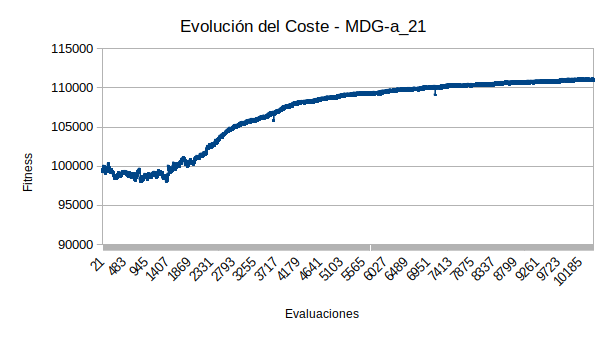
\includegraphics[scale=0.9]{../output/exp2/evalMDG}
		%\caption{my-captino} \label{my-label}
	\end{figure}
	
	\begin{figure}[H] 
		\centering
		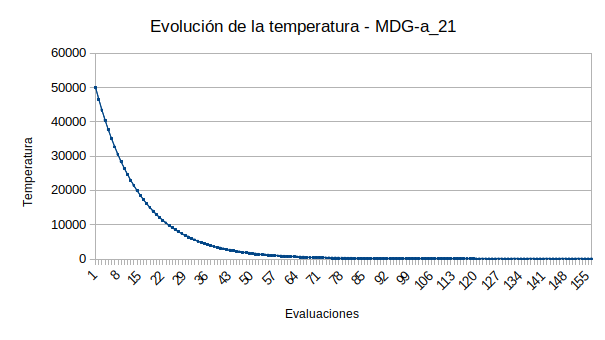
\includegraphics[scale=0.9]{../output/exp2/tempMDG}
		%\caption{my-captino} \label{my-label}
	\end{figure}
	
	\begin{figure}[H] 
		\centering
		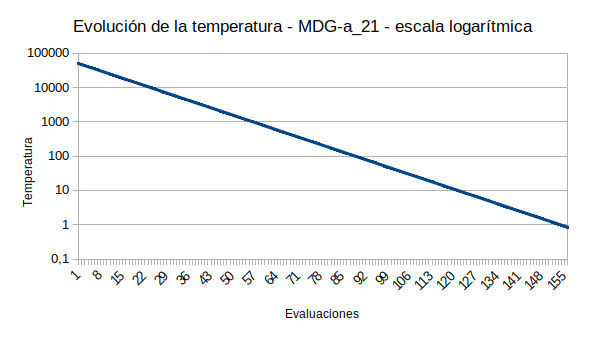
\includegraphics[scale=0.9]{../output/exp2/LtempMDG}
		%\caption{my-captino} \label{my-label}
	\end{figure}

	\begin{figure}[H] 
		\centering
		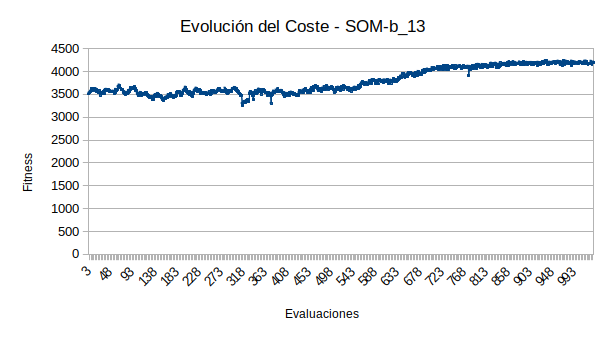
\includegraphics[scale=0.9]{../output/exp2/evalSOM}
		%\caption{my-captino} \label{my-label}
	\end{figure}
	
	\begin{figure}[H] 
		\centering
		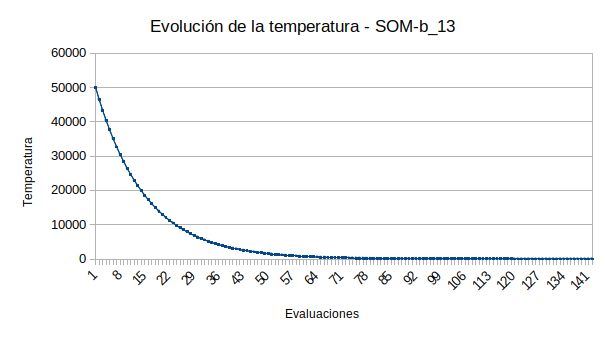
\includegraphics[scale=0.9]{../output/exp2/tempSOM}
		%\caption{my-captino} \label{my-label}
	\end{figure}
	
	\begin{figure}[H] 
		\centering
		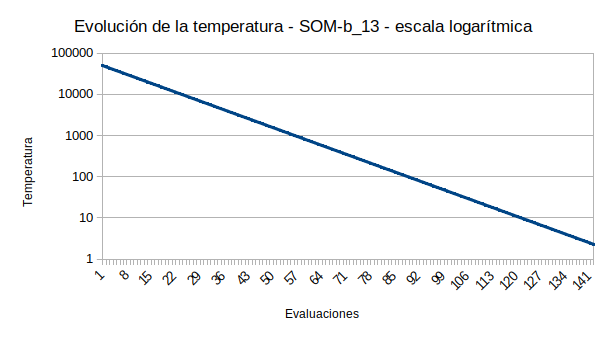
\includegraphics[scale=0.9]{../output/exp2/LtempSOM}
		%\caption{my-captino} \label{my-label}
	\end{figure}

	\paragraph{ Análisis } \ \\	

	En primer lugar observamos que el descenso de la temperatura en ambos casos es el esperado, lo hace según una progresión geométrica y de forma constante. Si bien este resultado no nos sorprende, si que debería hacerlo la precisión con la que el estudio realizado en la sección \ref{procedimiento3} se adapta al caso del problema: el número de enfriamientos no varía significativamente (alrededor de un 5\% de un caso a otro), y la temperatura final se acerca considerablemente a mínimo impuesto ($0.001$). \\
	
	Observando la evolución del $fitness$ en las distintas gráficas vemos como en numerosas ocasiones el coste de la solución en estudio desciende, pero esto ocurre con cada vez menos frecuencia conforme disminuye la temperatura, como cabría esperar. Se observa además un estancamiento hacia el final de la ejecución de ambos algoritmos, propiciando que el algoritmo pare antes de que se reduzca por completo la temperatura. \\
	
	Damos finalmente respuesta a la pregunta que originó este experimento. Si bien el número total de evaluaciones es francamente bajo, la evolución del $fitness$ y el estancamiento final no nos dan indicio de una convergencia prematura, si bien es cierto que podríamos reajustar los valores para permitir una mayor variación e intentar explorar más el espacio de soluciones. \\
	
	Debido a la falta de tiempo no me ha sido posible realizar más experimentos, como podrían haber sido la alteración de los parámetros del $ES$ (en particular el número de éxitos), o la evolución del $ILS-ES$.

\end{document}